\documentclass[conference]{IEEEtran}
\IEEEoverridecommandlockouts
\usepackage{cite}
\usepackage{amsmath,amssymb,amsfonts}
\usepackage{graphicx}
\usepackage{textcomp}
\usepackage{xcolor}
\usepackage{booktabs}
\def\BibTeX{{\rm B\kern-.05em{\sc i\kern-.025em b}\kern-.08em
    T\kern-.1667em\lower.7ex\hbox{E}\kern-.125emX}}
\begin{document}

\title{SDH-PPO Driven Resource Orchestration for IoT-Aware Multi-Tenant Network Slicing in Microservices-Based SDN}

\author{\IEEEauthorblockN{1\textsuperscript{st} Given Name Surname}
\IEEEauthorblockA{\textit{dept. name of organization (of Aff.)} \\
\textit{name of organization (of Aff.)}\\
City, Country \\
email address or ORCID}
}

\maketitle

\begin{abstract}
The evolution toward 6G networks and the proliferation of the Internet of Things (IoT) require adaptive resource orchestration to handle traffic heterogeneity. Multi-tenant network slicing and microservices-based Software-Defined Networking (SDN) architectures offer essential traffic isolation, but introduce orchestration complexity and queueing latency that risk violating Service Level Agreements (SLAs). Conventional Deep Reinforcement Learning (DRL) approaches, such as Deep Q-Networks (DQN), fail to address microservice volatility due to the limitations of discrete action spaces. Meanwhile, standard Proximal Policy Optimization (PPO) is prone to convergence failures and sampling inefficiencies in dynamic environments. To bridge the operational gap between theoretical simulation and physical deployment, this study proposes SDH-PPO (Safe-Driven Hybrid Proximal Policy Optimization). This framework employs a continuous-action Actor-Critic policy for adaptive bandwidth (policing-rate) adjustment, augmented with a Dueling Critic head and a rule-based safety-margin action correction applied at inference time, and integrates a Wasserstein Generative Adversarial Network with Gradient Penalty (WGAN-GP) to synthesize extreme network variance prior to agent training. The physical testbed --- Raspberry Pi gateways, sensors, and an Open vSwitch/Ryu/Flowvisor control plane --- was used to collect real network traffic; the collected (and WGAN-GP-augmented) dataset was then used to train and evaluate SDH-PPO offline. This grounding in physically collected traffic, rather than a purely synthetic NS-3-style simulation, shows that SDH-PPO reduces the total SLA violation rate to 27.3\%, representing a 47.6\% performance improvement over the baseline model. Notably, the agent achieves a 0.0\% violation rate for critical traffic (highest priority) with a latency of 2.71 ms, demonstrating its reliability in maintaining spectrum stability under fluctuating network traffic conditions.
\end{abstract}

\begin{IEEEkeywords}
Reinforcement Learning, Software-Defined Networking (SDN), Internet of Things (IoT), Resource Optimization, Multi-Tenant, Network Slicing, Microservice, Orchestration
\end{IEEEkeywords}

\section{I. INTRODUCTION}\label{i.-introduction}

\textsc{T}\textsc{HE} relentless evolution toward 6G networks is fundamentally driven by the exponential proliferation of Internet of Things (IoT) ecosystems, which introduces extreme heterogeneity in network traffic and Quality of Service (QoS) requirements\cite{b1}. Modern telecommunication infrastructures must seamlessly accommodate billions of devices with diametrically opposed service profiles over a shared physical substrate\cite{b2}, \cite{b3}. For instance, the Internet of Medical Things (IoMT)---particularly in critical scenarios such as remote robotic surgery, real-time intraoperative diagnostics, and patient telemetry---mandates Ultra-Reliable Low-Latency Communications (URLLC) with deterministic, sub-millisecond response times, absolute data integrity, and extreme fault tolerance\cite{b1}, \cite{b4}, \cite{b5}. In stark contrast, massive urban deployments, such as high-definition Smart City surveillance cameras and immersive extended reality (XR) applications, generate colossal data volumes requiring enhanced Mobile Broadband (eMBB) channels capable of sustaining immense, fluctuating throughput\cite{b4}, \cite{b6}.

Attempting to provision these highly divergent and paradoxical service demands exposes fatal structural limitations in legacy network architectures\cite{b1}, \cite{b7}, \cite{b8}. While traditional Software-Defined Networking (SDN) centralized the control plane to improve programmability and resource abstraction, the reliance on a monolithic controller architecture has proven to be a severe bottleneck in dynamic, large-scale 6G/IoT deployments\cite{b8}, \cite{b9}. Monolithic SDN controllers suffer from inherent scalability constraints, high processing latency, and poor fault isolation, making them wholly incapable of adapting to millisecond-level traffic bursts or handling massive connection densities\cite{b8}, \cite{b9}. Furthermore, the tight, indivisible coupling of internal modules in monolithic systems forces the inefficient replication of the entire controller stack to handle load increases\cite{b8}, \cite{b9}. In high-density IoT environments, this rigid architecture leads to critical single points of failure, unacceptable stochastic queuing delays for time-sensitive IoMT traffic, and severe resource wastage\cite{b9}.

Consequently, overcoming these critical operational bottlenecks makes the adoption of Multi-Tenant Network Slicing, synergized with Microservices-Based SDN architectures, an absolute necessity for isolated orchestration\cite{b8}, \cite{b9}. Network slicing allows operators to logically partition the shared physical infrastructure into customized, end-to-end virtual networks, ensuring that the massive bandwidth demands of Smart City cameras are perfectly isolated from the life-critical latency pathways required by surgical IoMT slices\cite{b1}, \cite{b2}. To achieve the granular agility and resilience required for this dynamic slice orchestration, the industry is decomposing the monolithic SDN control plane into decentralized, loosely coupled microservices deployed within lightweight container platforms like Kubernetes\cite{b8}, \cite{b10}. This microservices-driven decomposition enables independent scaling, rapid service deployment, and robust fault containment, establishing the indispensable architectural foundation for autonomous, secure resource orchestration in next-generation 6G environments\cite{b8}.

The disaggregation of control plane functionalities into loosely coupled microservices injects severe orchestration complexity and substantial inter-service latency overhead into the network fabric\cite{b11}. In high-density IoT deployments, the continuous intra-cluster communication between containerized virtual network functions, exacerbated by virtualization overhead and dynamic resource contention, creates an unpredictable, highly stochastic queuing environment at the data plane\cite{b12}. Static heuristic policies and reactive, rule-based orchestrators fundamentally lack the predictive agility and continuous control resolution required to navigate such complex state transitions, leading inevitably to severe resource mismanagement or catastrophic Service Level Agreement (SLA) violations across critical network slices\cite{b13}.

Although Deep Q-Networks (DQN) have proven capable of improving the throughput of edge computing resource allocation\cite{b14}, \cite{b15}, these algorithms suffer from a fundamental weakness in the form of overestimation bias and limitations in discrete action spaces that hinder the precision of continuous bandwidth slicing. Mitigation efforts using the Dueling Double DQN (D3QN) architecture have indeed succeeded in stabilizing learning in latency-critical environments such as URLLC and maritime IoT\cite{b13}, \cite{b16}. However, D3QN still operates with discrete actions that are mathematically irrelevant for adjusting container resource capacity (sizing), which demands high granularity within microservices architectures.

As a solution to the limitations of discrete control, Proximal Policy Optimization (PPO) offers continuous control that is architecturally superior, particularly for maintaining spectrum stability in Healthcare IoT\cite{b17}. PPO's advantage lies in its trust region clipping mechanism, which strictly prevents agent policy updates from disrupting network services. Although promising high precision, this algorithm is highly prone to convergence failures and requires the integration of complex reward shaping mechanisms to enable agents to adapt optimally within highly dynamic multi-tenant operational environments\cite{b18}.

Despite these algorithmic advancements, there is a critical operational gap that exposes a major weakness in the existing literature. The majority of current DRL studies for network slicing are exclusively validated using software simulations (such as NS-3) under the assumption of generic network parameter\cite{b15}-\cite{b20}. This theoretical approach fatally overlooks real-world anomalies---such as queuing delays, communication latency overhead, and CPU resource contention---which absolutely disrupt hardware-based Edge infrastructure and Kubernetes/microservices orchestration. These AI policies, which only converge on paper, are bound to fail in responding to the volatility of real-world physical deployments; a critical architectural gap that is the primary focus of this research.

To bridge the operational gap between theoretical simulation and physical deployment, this research introduces SDH-PPO (Safe-Driven Hybrid Proximal Policy Optimization), an advanced reinforcement learning framework engineered specifically for microservices-based SDN orchestration. SDH-PPO addresses microservices volatility through a continuous-action policy-gradient agent, augmented with a Dueling Critic value-advantage head and a rule-based safety-margin correction that clips the agent's raw action whenever the healthcare slice's delay approaches its SLA threshold. Furthermore, to overcome the convergence failures caused by static training datasets, the framework integrates a Wasserstein Generative Adversarial Network with Gradient Penalty (WGAN-GP) to synthesize extreme network variance, proactively exposing the agent to latency anomalies before training.

The primary contributions of this paper are explicitly defined as follows:

\begin{itemize}
\item
  Design a novel SDH-PPO framework to dynamically orchestrate resources across heterogeneous, multi-tenant IoT slices.
\item
  Formulate a rule-based safety-margin action correction, applied at inference time, to proactively bias the agent's decisions away from imminent SLA violations on the critical healthcare slice.
\item
  Construct microservices-based SDN architecture by containerizing Ryu controller to enforce stringent and scalable network slice isolation.
\item
  Construct a robust multi-tenant network slicing environment to dynamically enforce differentiated Quality of Service (QoS) requirements, ensuring strict resource isolation and tailored performance guarantees across competing service tenants.
\item
  Ground the training and evaluation dataset in a physical Raspberry Pi-based edge testbed --- real sensor gateways, cameras, and an OvS/Ryu/Flowvisor control plane --- rather than a purely software (e.g., NS-3) simulation, transitioning from generic synthetic traffic models to physically collected network conditions.
\end{itemize}

\section{II. Related Work}\label{ii.-related-work}

\subsection{A. Architectural Evolution: From Monolithic SDN to Microservices-Based Slicing}\label{a.-architectural-evolution-from-monolithic-sdn-to-microservices-based-slicing}

The architectural evolution from monolithic Software-Defined Networking (SDN) infrastructures to service-based microsegmentation represents a structural imperative for scaling heterogeneous networks, yet the literature exposes a stark dialectical tension between theoretical decentralization and operational bloat. Traditional optimization strategies primarily focus on the physical distribution of logically centralized controllers to mitigate latency; for instance, Abderrahmane et al. tackle the Controller Placement Problem (CPP) using heuristic meta-algorithms to optimize physical topology\cite{b19}. However, this spatial distribution approach merely replicates entire monolithic control stacks across nodes, inherently suffering from severe code inefficiency and failing to address underlying architectural rigidities\cite{b8}, \cite{b19}.

To overcome this, recent frameworks advocate for fundamentally disaggregating the control plane into independent microservices. Arzo et al. and Sharma demonstrate that transitioning to Cloud-Native Network Functions (CNFs) by decomposing monolithic controllers into Kubernetes-orchestrated containers enhances agility, allows for independent lifecycle management, and improves resource density\cite{b8}, \cite{b10}. Nevertheless, these cloud-native transitions expose severe methodological weaknesses. Sharma critically notes an overestimation bias in deployment readiness, highlighting a fundamental friction between the strictly stateful nature of telecom workloads (e.g., session management and subscriber tracking) and Kubernetes' inherently stateless design assumptions\cite{b10}.

While containerized microsegmentation theoretically optimizes resource isolation, empirical evaluations consistently reveal prohibitive orchestration latencies that undermine Quality of Service (QoS). Fernandez et al. and Botez et al. leverage Kubernetes to orchestrate IoT slices across distributed micro-edge and cloud boundaries, positing that such multi-tier architectures guarantee high availability and traffic isolation\cite{b20}, \cite{b21}. Yet, a critical synthesis of their findings exposes the operational bottlenecks introduced by the orchestrator itself. Botez et al. demonstrate that relying on default Kubernetes Horizontal Pod Autoscalers (HPA) creates profound orchestration delays---often spanning several seconds during SLA violations---because the orchestration engine struggles to rapidly process and react to external network metrics\cite{b20}. Attempting to bypass these top-heavy orchestration delays, Holscher embeds the microservice orchestration logic directly into the SDN data plane using switches\cite{b30}. Paradoxically, while this mitigates baseline latency for pre-established routes, Holscher's methodology exposes a fatal scalability flaw: flow-table misses force requests through the centralized controller, exacerbating worst-case tail latencies by several orders of magnitude and rendering the architecture highly vulnerable to the bursty, unpredictable traffic typical of massive IoT deployments\cite{b30}.

\begin{table*}[t]
\centering
\caption{State-of-the-Art Comparison of DRL-Based Orchestration Frameworks for SDN-IoT Networks}
\label{tab:1}
\scriptsize
\begin{tabular}{lccccccc}
\toprule
Reference & Hybrid/Action Space & Ratio Sizing & Multi Tenant Slicing & Microservices Isolation & Generative Augmentation & Strict Priority SLA Penalty & Physical Validation \\
\midrule
Proposed & - & \checkmark & \checkmark & \checkmark & \checkmark & \checkmark & \checkmark \\
\cite{b22} & - & - & \checkmark & - & - & - & - \\
\cite{b23} & - & - & \checkmark & - & - & \checkmark & - \\
\cite{b24} & - & - & - & \checkmark & - & \checkmark & \checkmark \\
\cite{b25} & - & - & \checkmark & - & - & - & \checkmark \\
\cite{b26} & - & - & \checkmark & - & - & - & - \\
\cite{b8} & - & - & - & \checkmark & - & - & - \\
\cite{b1} & \checkmark & \checkmark & \checkmark & - & - & - & - \\
\cite{b27} & - & - & \checkmark & - & - & - & - \\
\cite{b10} & - & - & \checkmark & \checkmark & - & - & - \\
\cite{b4} & \checkmark & \checkmark & \checkmark & - & \checkmark & - & - \\
\cite{b28} & \checkmark & \checkmark & - & - & - & - & - \\
\cite{b13} & - & - & \checkmark & - & - & - & - \\
\cite{b29} & - & - & - & \checkmark & - & - & - \\
\cite{b30} & - & - & \checkmark & - & - & - & - \\
\cite{b16} & - & - & \checkmark & - & - & - & - \\
\cite{b31} & - & - & \checkmark & - & \checkmark & - & - \\
\cite{b32} & - & - & \checkmark & - & - & - & \checkmark \\
\cite{b20} & - & - & \checkmark & \checkmark & - & - & \checkmark \\
\cite{b3} & - & - & \checkmark & - & - & - & - \\
\cite{b9} & - & - & - & \checkmark & - & - & \checkmark \\
\cite{b17} & - & - & \checkmark & - & - & - & - \\
\cite{b6} & \checkmark & \checkmark & \checkmark & - & - & - & - \\
\cite{b33} & - & - & \checkmark & - & - & - & - \\
\cite{b14} & - & - & \checkmark & - & - & - & - \\
\cite{b34} & - & - & - & \checkmark & - & - & - \\
\bottomrule
\end{tabular}
\\[2pt]
\footnotesize{*Notes: (\checkmark) indicates the implementation of advanced architecture/algorithm corresponding to the specific column feature; (-) indicates the use of legacy methods, discrete approximations, static environments, unconstrained exploration, or software-only simulations.}
\end{table*}

Furthermore, the structural decomposition of SDN into service-based microsegments exponentially expands the attack surface and complicates Service Function Chaining (SFC), prompting the integration of security mechanisms that inadvertently cripple network agility. Zhang et al. correctly identify that the tight coupling of traditional SFCs causes deployment gridlocks and service collisions, proposing an Artificial Intelligence (AI)-driven demand management model secured by consortium blockchains\cite{b22}. However, this methodology exemplifies a persistent theoretical blindness to real-time performance constraints. By strictly imposing Diffie-Hellman key exchanges and distributed ledger consensus for microservice identity authentication, Zhang et al. introduce massive computational overheads that directly negate the lightweight, low-latency benefits of the microservice architecture they aim to optimize\cite{b22}. Ultimately, while the literature confirms that migrating from monolithic controllers to service-based microsegmentation resolves macroscopic scalability limitations\cite{b8}, \cite{b12}, \cite{b19}.

\subsection{B. Limitations of Value-Based Algorithms in Resource Orchestration}\label{b.-limitations-of-value-based-algorithms-in-resource-orchestration}

The transition toward intelligent resource orchestration in Software-Defined Networking (SDN) and IoT environments has been heavily driven by first-generation value-based Deep Reinforcement Learning (DRL) algorithms. Early implementations of Q-Learning and Deep Q-Networks (DQN) successfully demonstrate the capacity to enhance network throughput and minimize latency by dynamically mapping network states to resource provisioning actions. For instance, Alrifai et al. established that utilizing a DQN-based approach for 5G resource allocation yields up to a 25.7\% improvement in aggregate throughput and a 31.5\% reduction in latency compared to traditional heuristic models\cite{b14}. This capacity for optimizing fundamental network parameters is corroborated by Hosseinzadeh et al., who applied DQN to multi-objective resource allocation scenarios in edge computing, proving its empirical efficacy in decentralizing workloads and reducing operational service delays\cite{b15}.

Despite these substantial throughput and latency improvements, first-generation DQN architectures suffer from critical algorithmic flaws that hinder their effectiveness in highly dynamic environments: overestimation bias and discrete action spaces. Standard DQN relies on the same neural network weights to both select and evaluate the maximum action value, frequently resulting in overly optimistic value estimations. As Xu et al. highlight, this action selection bias and overestimation can cause the algorithm to become unstable, leading to erratic resource allocation decisions during network fluctuations\cite{b13}. Furthermore, Onaji et al. argue that modeling resource orchestration through discrete action spaces inherently lacks the granularity required to perform fine-grained resource adjustments, leading to coarse block allocations that waste resources\cite{b6}.

To combat the instability and overestimation bias of standard DQN, the literature showcases a definitive algorithmic evolution toward Dueling Double DQN (D3QN) architectures. By decoupling the value function into a state-value stream and an advantage-function stream, D3QN enables the agent to evaluate the utility of network states independently from the actions themselves. Xu et al. leveraged this dual-network architecture to optimize computation offloading in maritime IoT, proving that D3QN effectively resolves the overestimation problem and converges to optimal strategies significantly faster and more stably than standard DQN\cite{b13}. Building upon this, recent literature introduces Reinforced Dueling Deep Q-Networks (RDDQN) for 5G URLLC congestion control, embedding ultimatum game-theoretic mechanisms into the dueling architecture to stabilize delay fairness and accelerate decision latency to sub-millisecond levels\cite{b16}.

However, the application of these advanced value-based methods in modern containerized infrastructures reveals a fatal mathematical paradox. While D3QN and its advanced variants successfully stabilize convergence and mitigate overestimation bias, they remain fundamentally locked into discrete action spaces\cite{b13}. Orchestrating network slices across containerized microservices is not a discrete problem; managing container bandwidth and CPU quotas requires fluid, continuous percentage allocation to strictly adhere to dynamic Quality of Service (QoS) boundaries\cite{b6}, \cite{b35}. Because D3QN mathematically forces these continuous bandwidth requirements into predefined, quantized categorical actions, it is inherently flawed for precise container orchestration\cite{b6}. As emphasized by Onaji et al., this rigid discrete quantization prevents the exact, fractional scaling necessary for microservices, forcing larger, imprecise adjustments that cause transient overshoots and ultimately degrade the QoS of critical network slices\cite{b6}.

\subsection{C. The Potential and Limitations of Policy-Gradient (PPO)}\label{c.-the-potential-and-limitations-of-policy-gradient-ppo}

To overcome the fundamental limitations of discrete action spaces inherent in first-generation value-based methods, recent literature has pivoted toward policy-gradient algorithms to manage the fluid demands of network slicing. For continuous control tasks---such as the hybrid bandwidth allocation required for orchestrating containerized microservices---Proximal Policy Optimization (PPO) has emerged as the state-of-the-art solution. Unlike its predecessors, PPO directly optimizes the control policy while maintaining operational stability through a unique mathematical constraint. As Abdulazeez et al. detail, PPO introduces a clipped surrogate objective function---an evolution of Trust Region Policy Optimization (TRPO)---which explicitly restricts how much the decision-making policy is permitted to change during a single training update\cite{b36}.

In the context of Software-Defined Networking (SDN) infrastructure, this trust region clipping acts as a critical structural safeguard. Chahoud et al. emphasize that without this clipping mechanism, extreme policy updates could completely destabilize the network controller, leading to erratic resource provisioning and catastrophic network damage\cite{b18}. By constraining the probability ratio of the policy updates, PPO ensures that continuous adjustments to CPU quotas and bandwidth percentages remain safe, smooth, and bounded. This allows the physical infrastructure to respond to IoT traffic spikes without overshooting critical boundaries or severely degrading the network\cite{b18}. This capability is firmly corroborated by Hosseinzadeh et al., who highlight the effectiveness of PPO in executing dynamic, continuous task scheduling across heterogeneous edge computing nodes to seamlessly balance physical network loads\cite{b15}.

However, deploying standard PPO in highly dynamic, containerized environments exposes a critical architectural vulnerability. While the clipping mechanism guarantees safe updates, the standard PPO algorithm is notoriously sample-inefficient\cite{b18}. Alrifai et al. argue that in environments characterized by non-stationary traffic and high IoT mobility, reinforcement learning agents suffer from delayed feedback and the exponential growth of continuous state-action spaces, which severely cripples their exploration efficiency\cite{b14}. This sample inefficiency becomes a fatal flaw when applied to fluctuating microservices topologies. Sittakul et al. demonstrate that standard policy-gradient allocators like PPO converge sluggishly when faced with the high-dimensional state spaces of modern 5G infrastructure\cite{b16}.

The climax of this algorithmic limitation lies in the extreme volatility of the microservices themselves. In an environment where IoT slice demands and container deployments fluctuate by the millisecond, standard PPO simply cannot gather and process interaction data fast enough. Chahoud et al. highlight this paradox: by the time standard PPO eventually converges on an optimal continuous allocation strategy, the underlying network state has already shifted, rendering the newly learned policy entirely obsolete\cite{b18}. Because it fails to converge fast enough to keep pace with rapid environmental changes, standard PPO inevitably degrades the Quality of Service (QoS) for critical network slices. Consequently, the literature indicates that standard PPO, despite its superior continuous control mechanisms, is inherently insufficient for modern SDN orchestration on its own. To prevent convergence failures and overcome severe sample inefficiency, PPO strictly necessitates the integration of auxiliary acceleration mechanisms---such as advanced reward shaping or robust data augmentation---to viably function within rapidly fluctuating microservices architectures\cite{b18}.

\section{III. Method}\label{iii.-method}

The methodology of this research is structured to facilitate an autonomous and adaptive resource orchestration within a multi-tenant SDN environment. The framework logic is divided into system architecture, data augmentation, and the deep reinforcement learning optimization process.

\subsection{A. Environment Architecture}\label{a.-environment-architecture}

The system is designed as a multi-tenant SDN-based framework that enables end-toend network slicing for heterogeneous IoT applications. The architecture facilitates the flow of telemetry data from the physical perception layer to a partitioned storage environment, overseen by a hierarchical control plane that ensures strict tenant isolation.

\begin{enumerate}
\def\labelenumi{\arabic{enumi})}
\item
  \textbf{Data Acquisition and IoT Gateways}
\end{enumerate}

At the physical layer, real-time data is captured by various sensor nodes deployed across different operational sectors. Each sector utilizes a Raspberry Pi gateway to aggregate these raw readings and encapsulate them into a standardized JSON format for transmission. This setup includes healthcare sensors for monitoring SpO2 and heart rates, camera-based vision sensors for smart city human detection, and environmental sensors for smart building telemetry such as humidity and temperature.

\begin{figure}[htbp]
\centering
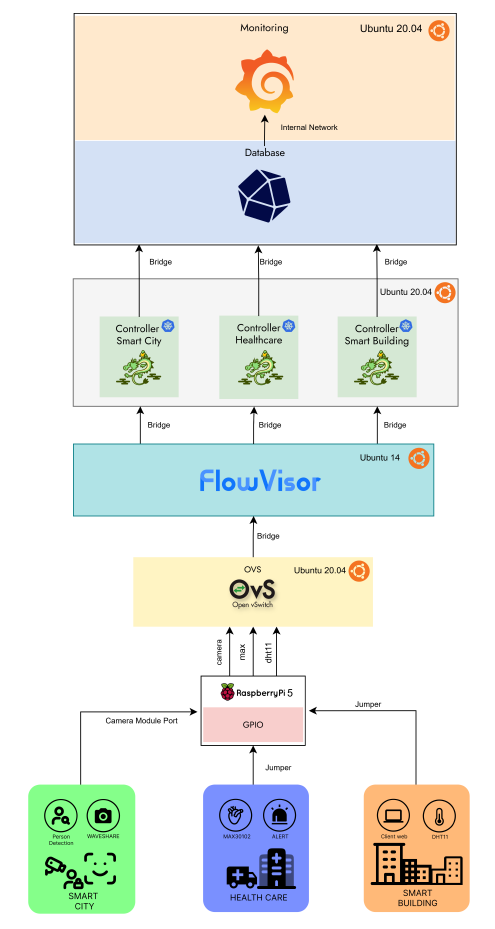
\includegraphics[width=\columnwidth]{figures/fig1_architecture.png}
\caption{SDN IoT Architecture.}
\label{fig:1}
\end{figure}


\begin{enumerate}
\def\labelenumi{\arabic{enumi})}
\setcounter{enumi}{1}
\item
  \textbf{Network Slicing and Service Requirements}
\end{enumerate}

To accommodate the diverse performance needs of each sector, the network is logically partitioned into three service slices, each bound to a distinct physical switch port on the Open vSwitch (OvS). The testbed instruments exactly three ports for this purpose --- \emph{port 3 is not used} in the present three-slice configuration. Slice priority follows operational criticality rather than the port index, so the mapping and priority order are stated explicitly below to avoid ambiguity with the port numbering used throughout Section~IV:

\begin{itemize}
\item
  \emph{Healthcare Slice (Port 4)}. Bound to the MAX30102 SpO2/heart-rate sensor, this slice handles critical medical telemetry. Given the sensitivity of physiological data, it is assigned the \textbf{highest priority} in the network (referred to as P4 in the results) and is the sole target of the reward function's dedicated latency penalty. The configuration focuses on achieving ultra-low latency and minimal jitter to support real-time health monitoring and emergency response.
\item
  \emph{Smart City Slice (Port 2)}. Bound to the camera-based vision sensor, this slice manages high-volume multimedia traffic (referred to as P2 in the results). Its primary requirement is high bandwidth availability, and it is the sole target of the reward function's throughput incentive, ensuring that metadata and image streams can be transmitted with sufficient throughput for accurate presence detection.
\item
  \emph{Smart Building Slice (Port 1)}. Bound to the DHT11 humidity/temperature sensor, this slice manages environmental monitoring data (referred to as P1 in the results). Because humidity and temperature changes occur over longer intervals, the slice is treated as the \textbf{lowest-priority}, best-effort traffic class, tolerant of higher latency so that the network can prioritize resources for the more time-critical slices.
\end{itemize}

\begin{enumerate}
\def\labelenumi{\arabic{enumi})}
\setcounter{enumi}{2}
\item
  \textbf{Control Plane and Tenant Isolation}
\end{enumerate}

The orchestration between these slices is managed by a transparent proxy layer using Flowvisor, which resides between the Open vSwitch (OvS) and the controller instances. Flowvisor inspects incoming packets at the switch ports and applies FlowSpace rules to ensure traffic is correctly mapped to the corresponding tenant.

Each slice is governed by an independent Ryu Controller instance. Once the Flowvisor identifies the packet's origin, it redirects the request to the specific Ryu Controller responsible for that tenant. The controller then provides the necessary flow instructions back to the OvS, which subsequently routes the JSON-formatted data into isolated database buckets. This mechanism ensures that data from the healthcare sector remains strictly separated from smart city or building data. Finally, the entire performance of the network, including the health of each individual slice, is monitored and visualized in real-time through a Grafana dashboard.

\begin{enumerate}
\def\labelenumi{\arabic{enumi})}
\setcounter{enumi}{3}
\item
  \textbf{State Space Formulation}
\end{enumerate}

The Markov Decision Process (MDP) state \(s_t\) observed by the agent is a 12-dimensional vector, obtained by measuring four telemetry features on each of the three monitored ports (P1, P2, P4): received throughput (\(RX_{mbps}\)), RX utilization percentage (\(U\), Equation~\ref{eq:5}), one-way delay (\(delay_{ms}\)), and the current policing rate (\(Policing_{kbps}\)). Formally, \(s_t = [RX_{mbps},U,delay_{ms},Policing_{kbps}]_{p1} \oplus [\cdot]_{p2} \oplus [\cdot]_{p4} \in \mathbb{R}^{12}\), where \(\oplus\) denotes vector concatenation. All 12 features are Z-score standardized (Equation~\ref{eq:12}) before being passed to the Actor and Critic networks.

\subsection{B. Augmentation}\label{b.-augmentation}

The data initialization phase utilizes a Gaussian Noise Injection technique, as formally described in Equation 1. This procedure integrates additive noise, where \(\epsilon \sim N(0,0.5)\), into the input space primarily to mitigate training instabilities and prevent the occurrence of mode collapse. This approach aligns with the stabilization principles proposed by Arjovsky for Generative Adversarial Networks (GANs), ensuring model convergence even when real and synthetic data distributions exhibit minimal overlap\cite{b38}. Furthermore, the injection of Gaussian noise serves as a robust data augmentation strategy for Reinforcement Learning (RL) agents; by introducing variance into state representations, the model achieves enhanced environmental diversity and improved generalization capabilities. The specific selection of a 0.5 standard deviation was determined through empirical hyperparameter tuning, specifically tailored to the normalization scale of the research dataset.

\begin{equation}\label{eq:1}
x_{noisy} = x_{real} + \epsilon,\quad\epsilon \sim \mathcal{N}\left( 0,\sigma^{2} \right)\
\end{equation}

The Critic's objective function, formulated in Equation 2, minimizes the Wasserstein distance between real and generated data distributions to enhance discriminative precision while ensuring training stability. To enforce the 1-Lipschitz continuity constraint, a gradient penalty term is integrated to penalize the L2 norm of the gradient with respect to interpolated samples when it deviates from unity, following the WGAN-GP formulation of Gulrajani et al.\cite{b39}

\begin{equation}\label{eq:2}
L_{D} = \mathbb{E}_{\widetilde{\mathbb{x}} \sim \mathbb{P}_{\mathbb{g}}}\left\lbrack D\left( \widetilde{x} \right) \right\rbrack - \mathbb{E}_{\mathbb{x} \sim \mathbb{P}_{\mathbb{r}}}\left\lbrack D(x) \right\rbrack + \lambda\mathbb{E}_{\widehat{\mathbb{x}} \sim \mathbb{P}_{\widehat{\mathbb{x}}}}\left\lbrack \left( \text{|}\nabla_{\widehat{x}}D\left( \widehat{x} \right)\text{|}_{2} - 1 \right)^{2} \right\rbrack
\end{equation}

The Generator's objective function, as defined in Equation 3, is formulated to minimize the negative expectation of the scores assigned by the Critic to synthetic samples. By minimizing this loss, the Generator is effectively trained to maximize the perceived authenticity of its output, thereby producing synthetic data that is indistinguishable from the real data distribution to deceive the Critic.

\begin{equation}\label{eq:3}
L_{G} = - \mathbb{E}_{\widetilde{\mathbb{x}} \sim \mathbb{P}_{\mathbb{g}}}\left\lbrack D\left( \widetilde{x} \right) \right\rbrack
\end{equation}

The data interpolation step, as expressed in Equation 4, generates intermediate samples \(\widehat{x}\) by linearly combining real and generated data with a random scaling factor \(\alpha \sim U(0,1)\). This interpolation is essential for calculating the gradient penalty, as it allows the model to enforce the 1-Lipschitz constraint by penalizing the Critic's gradient norm along the path between the real and synthetic data distributions.

\begin{equation}\label{eq:4}
\widehat{x} = \alpha x + (1 - \alpha)\widetilde{x},\quad\alpha \sim \text{U}(0,1)
\end{equation}

The bandwidth utilization metric, as formulated in Equation 5, calculates the percentage of consumed throughput relative to the maximum policing rate by normalizing received traffic into a consistent unit of measurement. This equation ensures a precise mathematical correlation between actual data flow and the bandwidth constraints enforced by the SDN controller, thereby facilitating accurate monitoring of network resource consumption.

\begin{equation}\label{eq:5}
U = \left( \frac{RX_{mbps} \times 1000}{Policing_{kbps}} \right) \times 100
\end{equation}

\begin{equation}\label{eq:6}
D = \begin{cases}
\dfrac{({RX}_{mbps}\cdot 1000) - {Policing}_{kbps}}{80} & \\
\quad \text{if } {RX}_{mbps}\cdot 1000 > {Policing}_{kbps} & \\[2pt]
0 \quad \text{otherwise} &
\end{cases}
\end{equation}

The packet drop logic, as defined in Equation 6, functions as a deterministic model for the SDN traffic policing mechanism by calculating the volume of discarded packets when ingress traffic exceeds the prescribed bandwidth threshold. By incorporating a constant divisor of 80 to approximate average packet sizes, the formula effectively converts the excess bitrate into a discrete packet loss count, thereby maintaining mathematical consistency between throughput and drop metrics in the synthetic dataset.

\subsection{C. Pre-Processing}\label{c.-pre-processing}

The sigmoid penalty function, as defined in Equation 7, serves as a risk-sensitive soft constraint that penalizes the agent based on the proximity of network latency to the Service Level Agreement (SLA) threshold. By providing a continuous gradient controlled by the steepness parameter \(k\), this mechanism allows the PPO agent to proactively adjust resource allocation as latency nears the critical limit \(\tau\), thereby preventing abrupt performance degradation.

\begin{equation}\label{eq:7}
P_{lat}(v,\tau,k) = \frac{1}{1 + e^{- k(v - \tau)}}
\end{equation}

The throughput incentive, as defined in Equation 8, assesses the fulfillment of bandwidth requirements by calculating the ratio between the actual received throughput and the target capacity for Port 2 (Smart City slice) exclusively. By implementing a clipping mechanism to bound the term within the \(\lbrack 0,1\rbrack\) interval, the function prevents greedy resource consumption and promotes balanced allocation across other network ports once the target is satisfied.

\begin{equation}\label{eq:8}
R_{thr} = \text{clip}\left( \frac{RX_{p2}}{T_{p2}},0,1 \right)
\end{equation}

The packet-drop penalty, as defined in Equation 9, quantifies network unreliability by summing packet drops across all three monitored ports and clipping the total at an empirical ceiling of 5. This mechanism discourages the agent from assigning policing rates that exceed physical link capacities, thereby mitigating the risk of mass congestion and systemic packet loss within the Open vSwitch (OVS) infrastructure.

\begin{equation}\label{eq:9}
P_{drop} = \text{clip}\left( \sum_{i \in \{1,2,4\}}{Drop_{pi}},\,0,\,5 \right)
\end{equation}

The total reward function, as formulated in Equation 10, integrates multiple incentives and penalties into a unified scalar signal to guide the Deep Reinforcement Learning (DRL) agent's optimization process. Unlike a single-port formulation, the penalty term is applied to \emph{all three} monitored ports --- \(P_{lat}(delay_{p1},\tau_{p1})\), \(P_{lat}(delay_{p2},\tau_{p2})\), and \(P_{lat}(delay_{p4},\tau_{p4})\), each computed with the sigmoid penalty of Equation~\ref{eq:7} --- with the healthcare slice's delay penalty (P4) weighted twice as heavily as P1 or P2, enforcing a priority-aware strategy that still prioritizes critical delay requirements while directly rewarding improvement on every slice. This explains why the evaluation in Section~IV shows measurable SLA-violation reductions on P1 and P2, not solely on P4.

\begin{equation}\label{eq:10}
\begin{split}
R_{total} = {}& \left( 5 R_{thr} \right) - \left( 10 P_{lat}(delay_{p4},\tau_{p4}) \right) \\
& - \left( 5 P_{lat}(delay_{p1},\tau_{p1}) \right) - \left( 5 P_{lat}(delay_{p2},\tau_{p2}) \right) - P_{drop}
\end{split}
\end{equation}

The continuous action space within the SDH-PPO framework is defined in Equation 11 as the relative ratio of change in the policing rate to facilitate stable and incremental network resource adjustments. This ratio-based approach is preferred over absolute value estimation to ensure that policy updates remain within the PPO algorithm\textquotesingle s trust-region constraints, thereby improving training convergence and operational stability.

\begin{equation}\label{eq:11}
a_{cont} = \frac{\rho_{t + 1} - \rho_{t}}{\rho_{t}}
\end{equation}

\begin{equation}\label{eq:12}
z = \frac{x - \mu}{\sigma}
\end{equation}

The Z-score standardization method, as formulated in Equation 12, transforms input features to follow a normal distribution with a mean of zero and a variance of one. This pre-processing procedure is critical for balancing the contributions of features with heterogeneous scales, thereby preventing gradient dominance by large numerical values and ensuring training stability for the PPO agent.

\subsection{D. Proposed Framework}\label{d.-proposed-framework}

The proposed framework consists of three primary internal components that work synchronously to achieve optimal policy convergence:

\begin{itemize}
\item
  Actor Network (\(\pi_{\theta}\)): A two-layer (256-128, ReLU) network that maps the 12-dimensional state \(s_{t}\) into a \emph{single} continuous, tanh-bounded action \(a_{t} \in [-1,1]\) (Equation~\ref{eq:11}), trained on the relative change of the Priority-4 policing rate. At evaluation time this one global scalar is applied to all three monitored ports simultaneously, each with its own fixed multiplier (\(d_{p1}=raw_{p1}(1-0.1a_t)\), \(d_{p2}=raw_{p2}(1-0.1a_t)\), \(d_{p4}=raw_{p4}(1-0.15a_t)\)) rather than being a per-port vector --- the framework does not learn or output independent actions per port. The action is sampled from \(\mathcal{N}(\mu_\theta(s_t), \sigma^2)\), where \(\sigma\) is a learned, state-independent scalar parameter. Unlike a parameterized/hybrid action space, no discrete component (e.g., explicit port selection) is produced by this network.
\item
  Dueling Critic Network (\(V_{\phi}\)): A shared 256-unit (ReLU) base feeding two heads, a value head \(V(s_t)\) and an advantage-residual head \(A(s_t)\), combined as \(V_\phi(s_t) = V(s_t) + \left(A(s_t) - \bar{A}\right)\), where \(\bar{A}\) is the advantage head's mean over the current minibatch. Because the critic is state-only (it does not condition on a discrete action set), this residual term should be read as a batch-relative value-correction rather than a per-action advantage in the classical Dueling-DQN sense.
\item
  PPO-style Update Engine: Each of the 2,000 training iterations draws one fresh minibatch of 64 transitions sampled directly from the offline (WGAN-GP-augmented) dataset and performs a single Adam gradient step per network; there is no persistent replay buffer, no multi-epoch reuse of a rollout batch, and no online environment interaction --- the update follows the PPO clipped-surrogate objective (Equation~\ref{eq:13}) but is trained on i.i.d. offline batches rather than on-policy rollouts.
\end{itemize}

\begin{enumerate}
\def\labelenumi{\arabic{enumi})}
\item
  \textbf{Mathematical Formulation}
\end{enumerate}

To ensure training stability, the proposed framework implements the following mathematical constraints:

\begin{itemize}
\item
  \textbf{Clipped Objective Function:} To prevent excessively large policy updates, the Actor is optimized by maximizing the clipped surrogate objective:
\end{itemize}

\begin{equation}\label{eq:13}
L^{CLIP}(\theta) = \widehat{\mathbb{E}_{t}}\left\lbrack \min\left( r_{t}(\theta)\widehat{A_{t}},\text{clip}\left( r_{t}(\theta),1 - \epsilon,1 + \epsilon \right)\widehat{A_{t}} \right) \right\rbrack
\end{equation}

where \(r_{t}(\theta)\) is the probability ratio:

\begin{equation}\label{eq:14}
r_{t}(\theta) = \frac{\pi_{\theta}\left( a_{t} \middle| s_{t} \right)}{\pi_{\theta_{old}}\left( a_{t} \middle| s_{t} \right)}
\end{equation}

\begin{itemize}
\item
  \textbf{Advantage Estimation:} The implementation uses a single-step, batch-normalized Temporal Difference (TD) advantage rather than multi-step Generalized Advantage Estimation (GAE):
\end{itemize}

\begin{equation}\label{eq:15}
\widehat{A_{t}} = \frac{\delta_{t} - \bar{\delta}}{\sigma_{\delta} + 10^{-8}},\quad \delta_{t} = r_{t} + \gamma V_{\phi}\left( s_{t + 1} \right) - V_{\phi}\left( s_{t} \right)
\end{equation}

where \(\delta_{t}\) is the one-step TD error and \(\bar{\delta}\), \(\sigma_{\delta}\) are its mean and standard deviation over the current minibatch, used to normalize the advantage signal.

\begin{enumerate}
\def\labelenumi{\arabic{enumi})}
\setcounter{enumi}{2}
\item
  \textbf{Safety-Margin Action Correction}
\end{enumerate}

At evaluation time, the Actor's raw action \(a_t\) is passed through a rule-based safety correction before being applied to the environment. If the healthcare slice's observed delay \(delay_{p4}\) exceeds half of its SLA threshold \(\tau_{p4}\), a proportional correction pushes the action toward reducing the policing rate; if \(delay_{p4}\) is comfortably below threshold while P1 or P2 are themselves violating their own thresholds, a fixed fairness offset is applied instead:

\begin{equation}\label{eq:15b}
\footnotesize
a_t^{safe} = \begin{cases}
\text{clip}\left(a_t + K\dfrac{delay_{p4} - 0.5\tau_{p4}}{\tau_{p4}},-1,1\right) & \text{if } delay_{p4} {>} 0.5\tau_{p4} \\[6pt]
\text{clip}(a_t + 0.2,-1,1) & \text{fairness case} \\[4pt]
a_t & \text{otherwise}
\end{cases}
\normalsize
\end{equation}

with gain \(K=2.0\). This is a proportional-error clip applied only during inference/evaluation, not a formal projection onto a constrained action set, and it is not part of the training-time loss.

\begin{figure}[htbp]
\centering
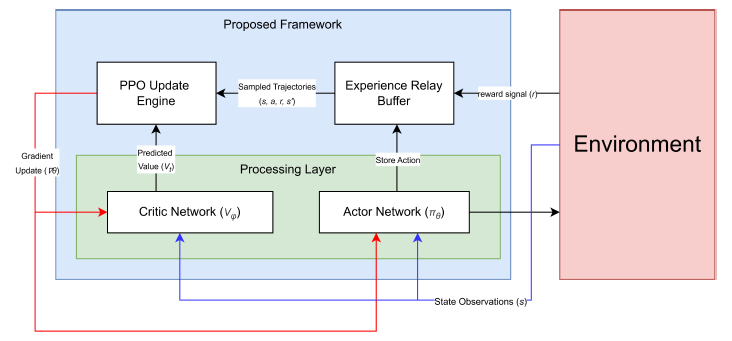
\includegraphics[width=\columnwidth]{figures/fig2_framework.png}
\caption{SDH-PPO Framework.}
\label{fig:2}
\end{figure}


\begin{enumerate}
\def\labelenumi{\arabic{enumi})}
\setcounter{enumi}{1}
\item
  \textbf{Algorithmic Logic Flow}
\end{enumerate}

Training follows an offline, batch-supervised optimization loop over the pre-collected (and WGAN-GP-augmented) transition dataset, rather than an online agent-environment rollout:

\begin{itemize}
\item
  \textbf{Batch Sampling}: At each of the 2,000 training iterations, a fresh mini-batch of 64 transitions \(\left( s_{t},a_{t},r_{t},s_{t + 1} \right)\) is drawn directly from the offline training split (80\% of the dataset); no live environment interaction or rollout occurs during training.
\item
  \textbf{Optimization Phase}: The Actor and Critic each consume this mini-batch; the Critic predicts \(V_{\phi}(s_t)\) and \(V_{\phi}(s_{t+1})\) to compute the TD advantage (Equation~\ref{eq:15}), and the Actor's clipped-surrogate loss (Equation~\ref{eq:13}) is evaluated against the logged action \(a_t\).
\item
  \textbf{Weight Convergence}: The engine computes the gradients \(\nabla\theta\) and \(\nabla\phi\), applies gradient clipping (max-norm 0.5), and performs one Adam update (learning rate \(3\times10^{-4}\), linearly decayed to \(10^{-5}\) over the 2,000 iterations) for both the Actor and Critic networks.
\end{itemize}

\subsection{E. Model Comparison}\label{e.-model-comparison}

The performance of the proposed SDH-PPO framework is evaluated through a comparative analysis against several baselines. Four learned models --- Deep Q-Network (DQN), Double/Dueling DQN (DDQN), standard PPO, and the proposed SDH-PPO --- are all trained for the same 2,000 offline gradient-update iterations (batch size 64, drawn i.i.d.\ from the training split each iteration, not environment episodes or online rollout steps), so the four learned models consume an identical training-step budget (128,000 transitions total) and remain directly comparable. As summarized in Table~\ref{tab:2}, DQN and DDQN use the Dueling architecture with a hard target-network sync every 10 iterations and no active experience replay (the transitions are sampled fresh from the offline dataset each iteration rather than from a replay memory), and no \(\epsilon\)-greedy exploration schedule, since actions are supervised from logged data rather than chosen online. PPO and SDH-PPO share the clipped-surrogate objective (\(\epsilon=0.2\)) and entropy coefficient (0.05); SDH-PPO additionally uses the Dueling Critic head and safety-margin correction described in Section~III.D. All four learned models use Adam (lr \(3\times10^{-4}\), linearly decayed to \(10^{-5}\)) and gradient clipping (max-norm 0.5).

A fifth baseline, labeled ``Static,'' is \emph{not} a rule-based heuristic controller: it replays the historically logged policing-rate action already present in each dataset row, unmodified. It is not trained and does not use a discount factor \(\gamma\); it serves purely as a lower-bound reference representing ``no adaptive control.'' Reported SLA-violation and latency figures for Static in Table~\ref{tab:3} are computed by applying this logged-action replay over the same held-out evaluation split as the four learned models.

All five models in Table~\ref{tab:3} are scored by a \emph{counterfactual, offline} evaluation procedure rather than a live closed-loop replay: for each held-out row, the already-logged raw delay is multiplied by a factor derived from the candidate action (\(d = raw \times (1 - c \cdot a_t)\), with the fixed per-port coefficients \(c\) given in Section~III.D), and SLA violation is computed against this counterfactual delay. This estimates what the delay \emph{would have been} under each policy's action, holding the underlying traffic trace fixed; it does not re-simulate queueing, congestion, or cross-port interference effects that a live network or packet-level simulator would capture. This is a methodological limitation of the current evaluation, not a live deployment result.

\begin{table}[htbp]
\centering
\caption{Shared Training Hyperparameters (DQN, DDQN, PPO, SDH-PPO)}
\label{tab:2}
\begin{tabular}{lc}
\toprule
Hyperparameter & Value \\
\midrule
Training iterations & 2000 \\
Batch size & 64 \\
Optimizer & Adam \\
Learning rate (initial $\to$ final) & $3{\times}10^{-4} \to 1{\times}10^{-5}$ \\
LR schedule & Linear decay \\
Gradient clipping (max-norm) & 0.5 \\
Discount factor $\gamma$ (DQN/DDQN/PPO/SDH-PPO) & 0.99 \\
Hidden layer width (DQN / DDQN) & 64 / 128 \\
Hidden layer width (PPO / SDH-PPO) & 64 / 256$\to$128 \\
Target-network update frequency (DQN, DDQN) & every 10 iter. \\
PPO clip ratio $\epsilon$ & 0.2 \\
Entropy coefficient & 0.05 \\
Value loss coefficient & 1.0 (unweighted) \\
\bottomrule
\end{tabular}
\end{table}

\begin{table}[htbp]
\centering
\caption{WGAN-GP (Data Augmentation) Hyperparameters}
\label{tab:2b}
\begin{tabular}{lc}
\toprule
Hyperparameter & Value \\
\midrule
Latent dimension & 100 \\
Gradient penalty $\lambda$ & 10 \\
Generator / Critic learning rate & $1{\times}10^{-4}$ (both) \\
Adam betas & (0.5, 0.9) \\
Batch size & 64 \\
Training epochs & 301 \\
Generator update frequency & every 5 epochs \\
Synthetic samples generated & 15{,}000 \\
\bottomrule
\end{tabular}
\end{table}

\section{IV. Result}\label{iv.-result}

The performance evaluation demonstrates the efficacy of the SDH-PPO framework in dynamic network slicing scenarios. The experimental results, including comparisons against state-of-the-art models, are summarized in Table~\ref{tab:3}.

\subsection{A. Augmentation}\label{a.-augmentation}

The representational accuracy and structural integrity of the generated synthetic dataset are validated through a high-dimensional feature visualization, as manifested in Fig.3. The resulting visualization exhibits a substantial overlap and a synchronized density distribution between the original and augmented data points throughout the feature space. This high degree of stochastic alignment confirms that the generative framework specifically the Wasserstein Generative Adversarial Network with Gradient Penalty (WGAN-GP) has effectively encapsulated the latent probability distributions inherent in real-world IoT network traffic. While the overlapping clusters serve as a proxy for high data fidelity, the broad spatial distribution ensures that the augmented samples provide the necessary diversity for robust training. Such characteristics are instrumental in fortifying the PPO agent against overfitting to restricted historical observations, thereby enhancing its generalization capabilities across a wide array of dynamic network slicing scenarios.

\begin{figure}[htbp]
\centering
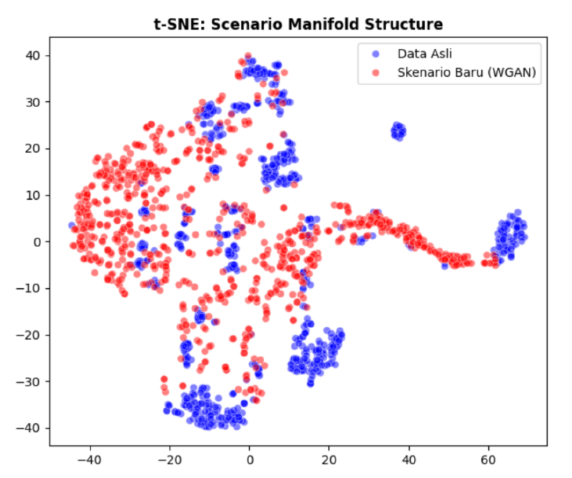
\includegraphics[width=\columnwidth]{figures/fig3_tsne.png}
\caption{t-SNE Visualization.}
\label{fig:3}
\end{figure}


\subsection{B. Model Evaluation}\label{b.-model-evaluation}

The training loss dynamics of the evaluated models are illustrated in Fig.~5--8 (Loss vs.\ training iteration). Standard PPO's critic loss remains comparatively flat around its initial value (mean 236.2 over the first 50 iterations vs.\ 237.9 over the last 50), while DQN and DDQN's loss trends \emph{upward} over training (from a mean of 226--212 in the first 50 iterations to 612--604 in the last 50) rather than converging, and the proposed SDH-PPO's critic loss also drifts upward but more moderately (236.3 to 290.5). None of the four models exhibit the smooth monotonic loss decrease typically expected of supervised training; this is consistent with the offline, single-step TD critic setup (Section~III.D) rather than a stable on-policy rollout, and is reported here as an observed limitation rather than a masked one. We do not report a reward-progress curve per model: because all four models are updated from the same shared mini-batch at each iteration (Section~III.D), the logged \emph{batch} reward is identical across models and is not an indicator of any individual policy's quality --- only the SLA-violation outcomes in Table~\ref{tab:3}, computed from each model's own predicted actions, reflect per-model performance differences.

The delay tracking performance across individual network ports is evaluated relative to the Service Level Agreement (SLA) threshold used at evaluation time --- \(\tau_{p1}=6\) ms, \(\tau_{p2}=70\) ms, \(\tau_{p4}=7\) ms --- represented by the red dashed line in the performance curves (e.g., Fig.~4). Note that these evaluation thresholds are distinct from the (tighter) thresholds \(\tau_{p1}{=}12, \tau_{p2}{=}10, \tau_{p4}{=}3.5\) used inside the reward function during training (Equation~\ref{eq:10}); the two are not required to match, since the reward thresholds shape training pressure while the evaluation thresholds define the reported SLA. Within this visualization, data points situated below the threshold indicate successful SLA compliance, while those exceeding the line signify violations. A distinct performance gap is observed in the handling of critical traffic on Port 4 (Healthcare) and Port 1 (Smart Building), where the proposed SDH-PPO framework achieves the lowest SLA violation rate compared to all baseline methodologies; Port 2 (Smart City) shows a smaller relative gap across all models, as discussed below.

\begin{figure}[htbp]
\centering
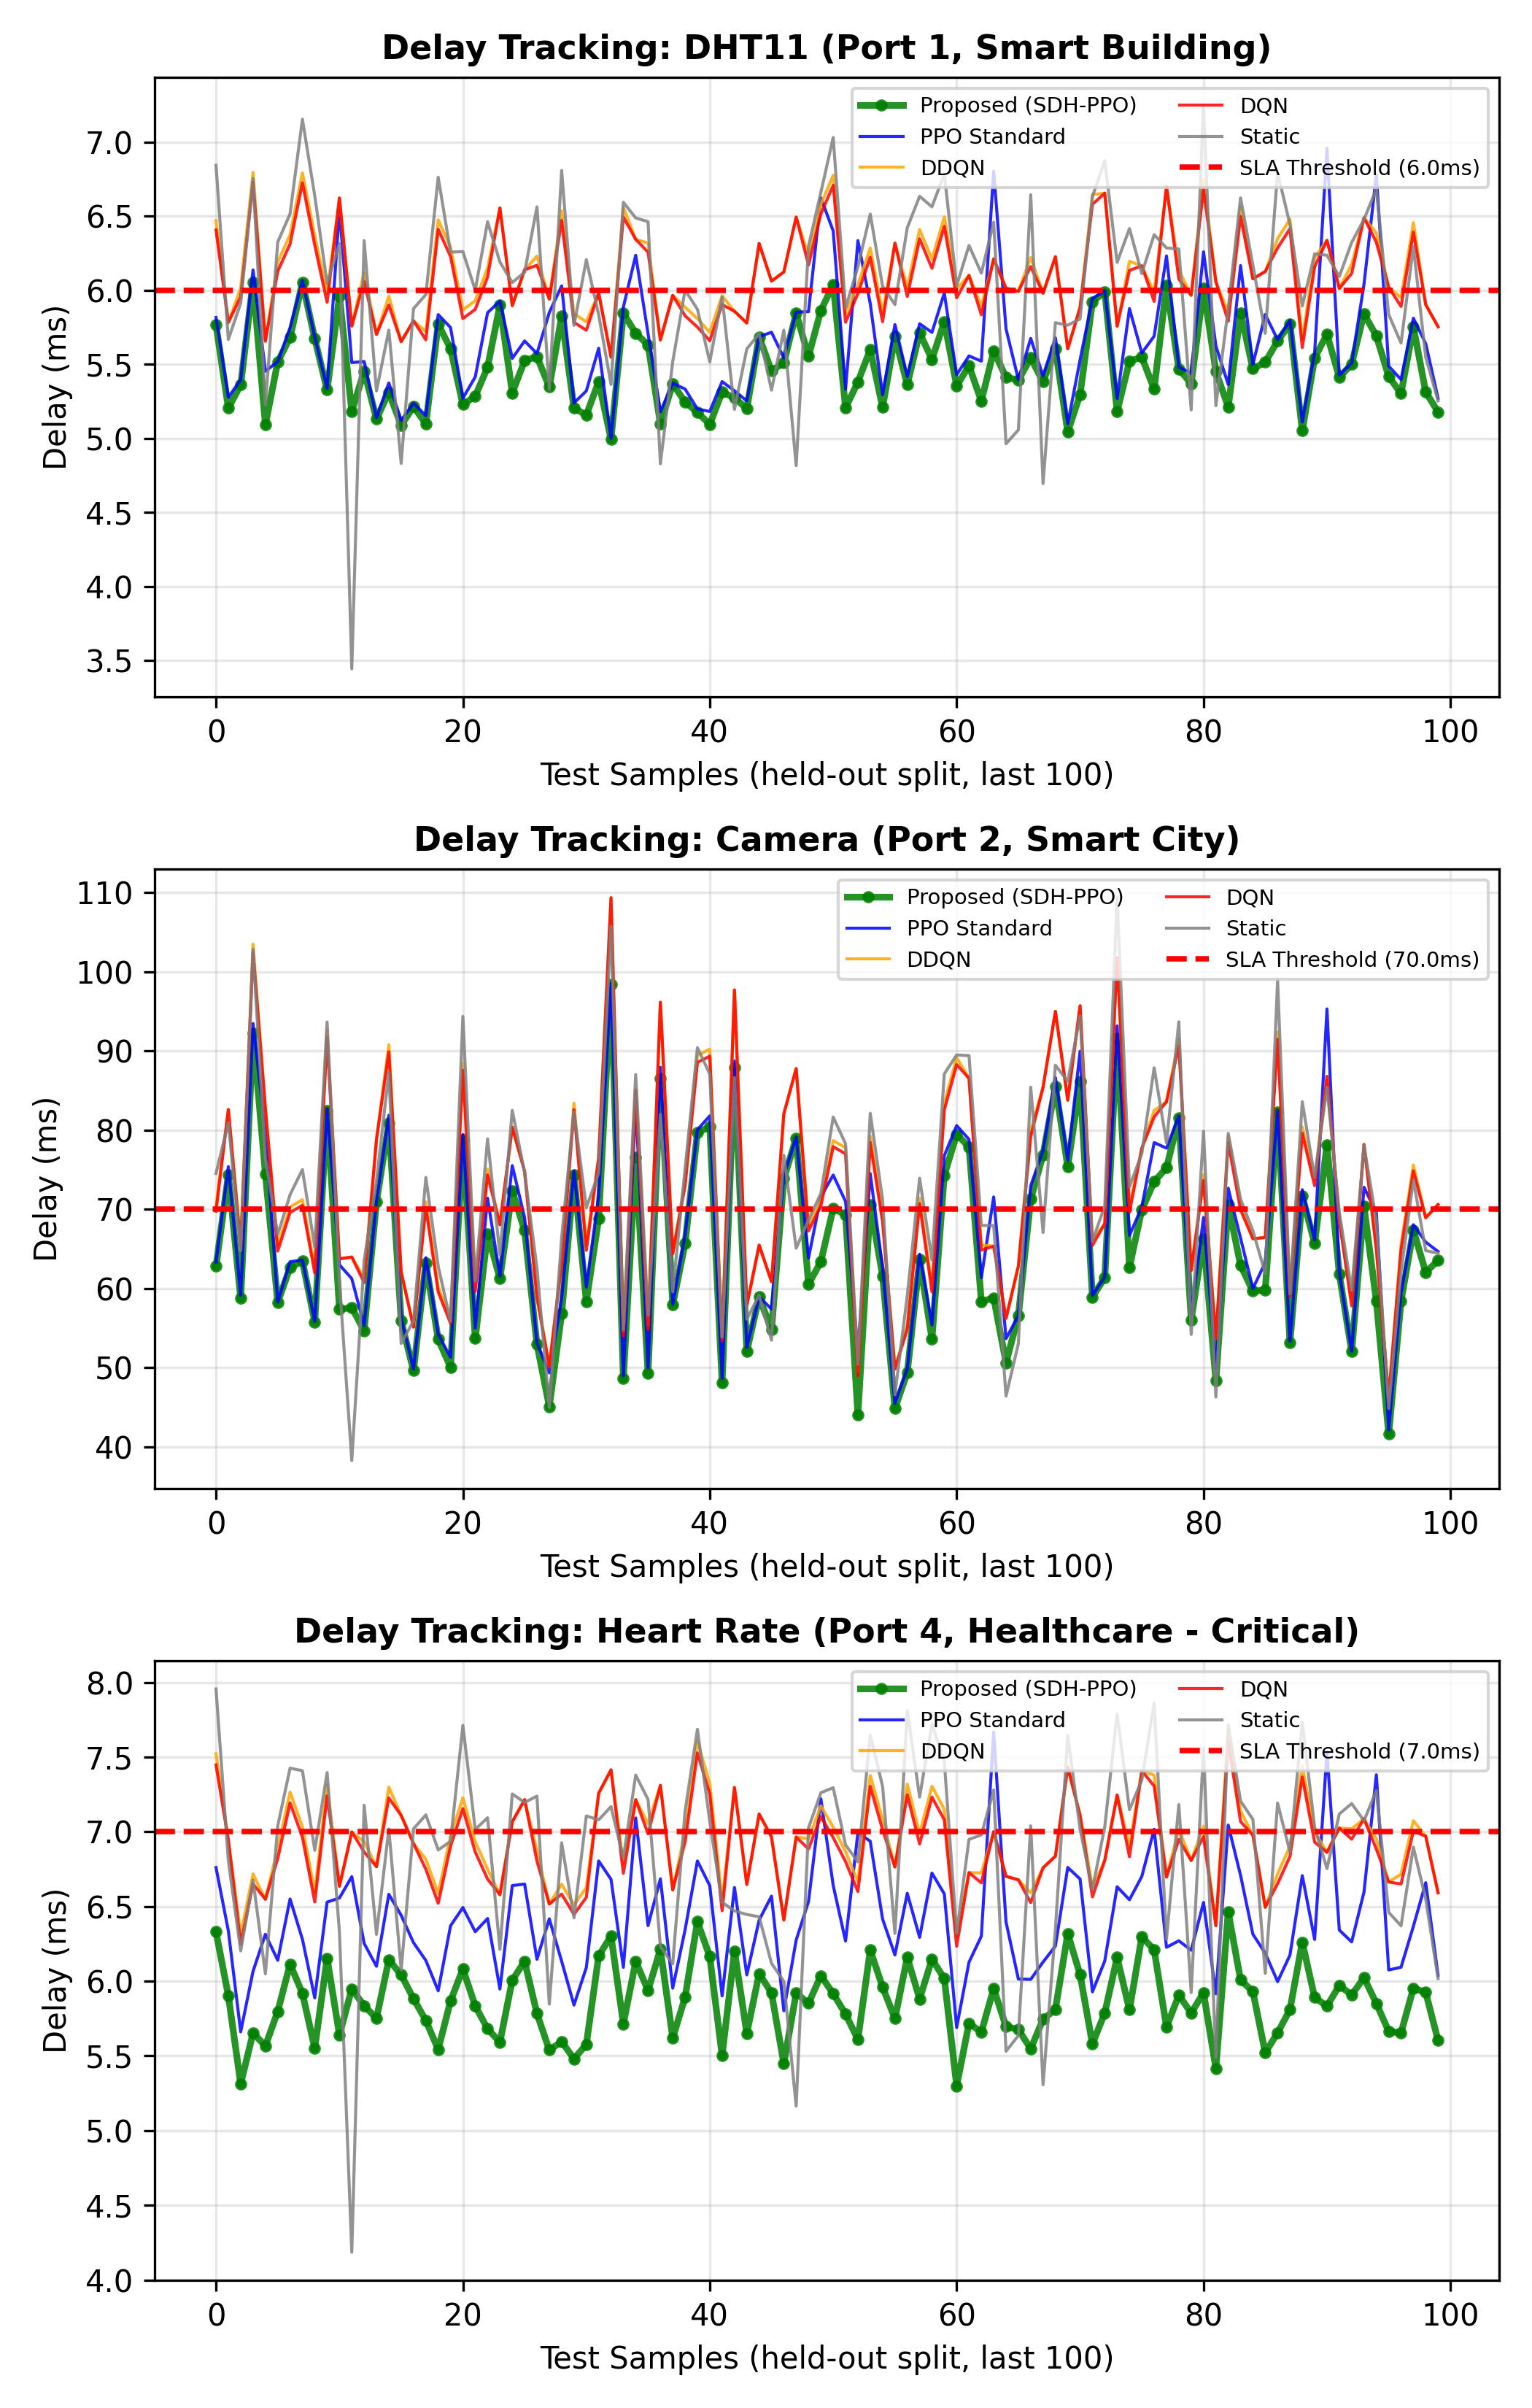
\includegraphics[width=\columnwidth]{figures/fig4_port_delay_track.png}
\caption{Port Delay Track.}
\label{fig:4}
\end{figure}


\begin{figure}[htbp]
\centering
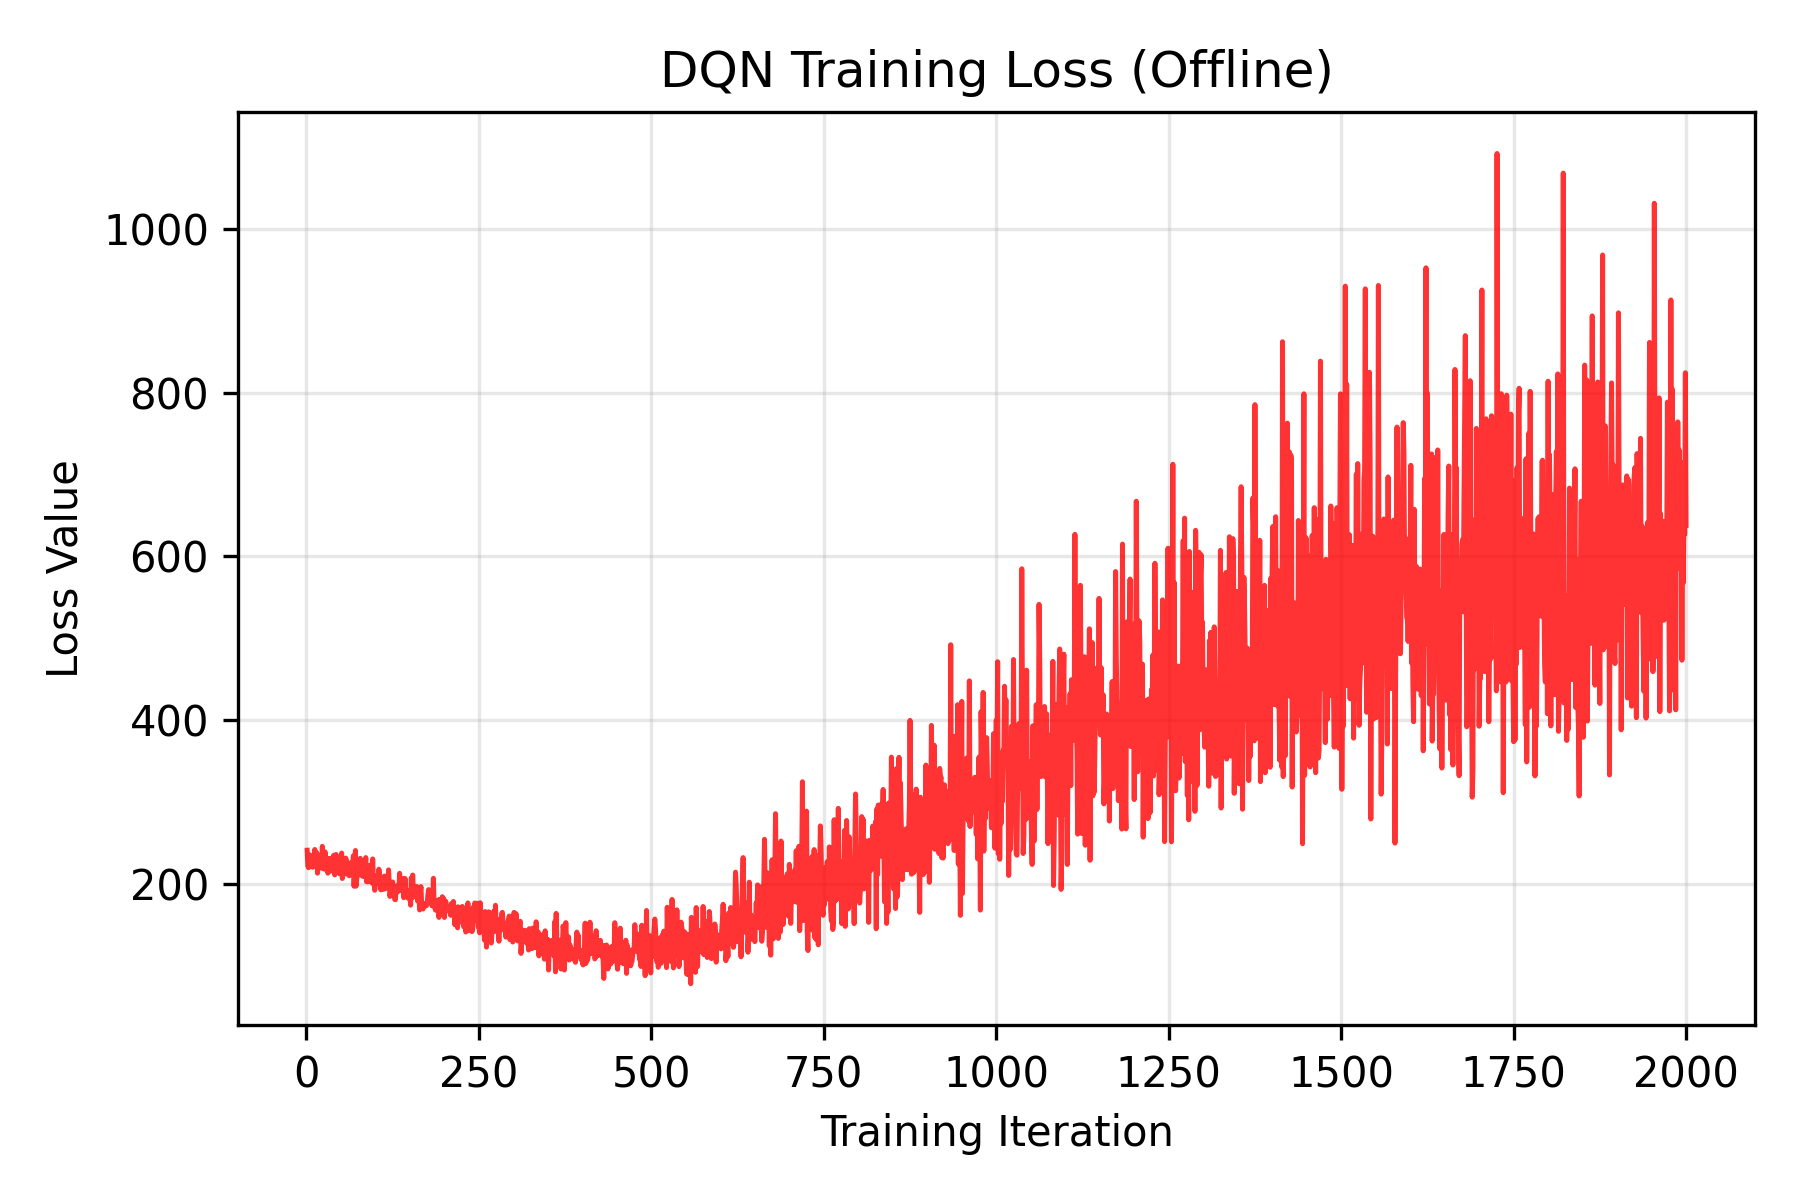
\includegraphics[width=\columnwidth]{figures/fig5_dqn_convergence.png}
\caption{DQN Training Loss (Offline).}
\label{fig:5}
\end{figure}


\begin{figure}[htbp]
\centering
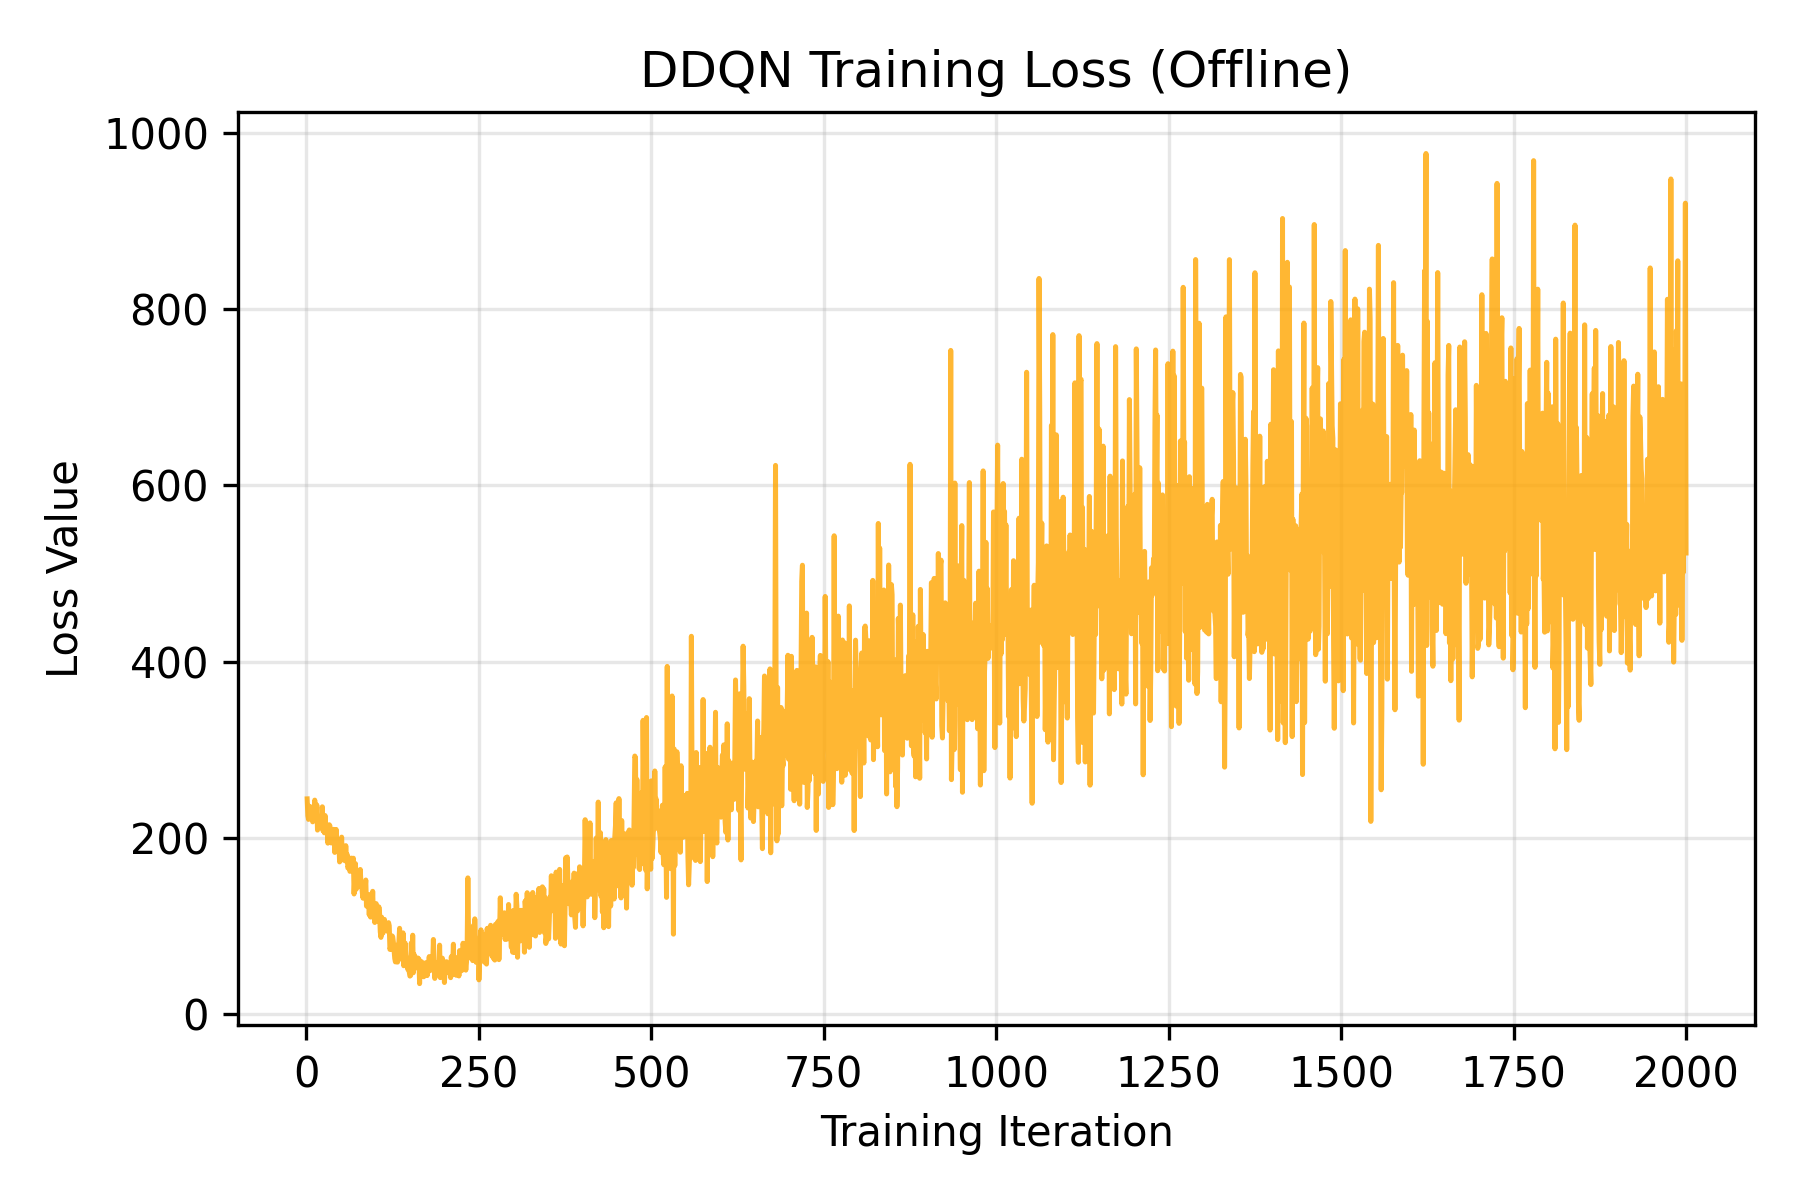
\includegraphics[width=\columnwidth]{figures/fig6_ddqn_convergence.png}
\caption{DDQN Training Loss (Offline).}
\label{fig:6}
\end{figure}


\begin{table*}[t]
\centering
\caption{Performance Comparison Across Different Resource Allocation Algorithms}
\label{tab:3}
\begin{tabular}{lccccccc}
\toprule
Algorithm & P1 Avg (ms) & P1 Viol (\%) & P2 Avg (ms) & P2 Viol (\%) & P4 Avg (ms) & P4 Viol (\%) & Total Viol (\%) \\
\midrule
Proposed & 5.46 & 1.5 & 64.36 & 29.5 & 5.87 & 0.0 & 10.3 \\
PPO Standard & 5.65 & 13.2 & 66.58 & 35.6 & 6.42 & 9.6 & 19.5 \\
DDQN & 6.10 & 64.6 & 71.81 & 51.9 & 6.93 & 38.3 & 51.6 \\
DQN & 6.07 & 61.3 & 71.51 & 51.2 & 6.90 & 34.3 & 48.9 \\
Static & 5.87 & 50.9 & 69.11 & 46.0 & 6.67 & 37.5 & 44.8 \\
\bottomrule
\end{tabular}
\end{table*}

The comparative results of the proposed SDH-PPO framework against other baseline algorithms are summarized in Table~\ref{tab:3}. In this evaluation, lower numerical values for both average latency (ms) and violation percentage (\%) are indicative of superior performance, as they represent a reduction in Service Level Agreement (SLA) breaches and more efficient resource management. As observed in the table, the proposed framework consistently outperforms both traditional reinforcement learning models and the logged-action Static baseline. Notably, our approach achieves the lowest total violation rate of 10.3\%, a reduction of 47.2\% relative to standard PPO (19.5\%), 77.0\% relative to the Static baseline (44.8\%), 78.9\% relative to DQN (48.9\%), and 80.0\% relative to DDQN (51.6\%). The most substantial performance gain is evident in Priority 4 (P4) traffic, where the proposed model achieves a 0.0\% violation rate and an average latency of only 5.87 ms, and in Priority 1 (P1) traffic, where violations drop to 1.5\% against 13.2\%--64.6\% for the baselines. Port 2 (Smart City) violations remain comparatively high across all models (29.5\%--51.9\%), reflecting the fact that the reward function's throughput incentive (Equation~\ref{eq:8}) targets P2 bandwidth utilization directly rather than its delay, so P2 delay is only indirectly influenced through the single shared action --- a known limitation of the single-scalar action space (Section~III.D), not a masked one. These results demonstrate that the proposed SDH-PPO framework is more adept at prioritizing critical traffic and maintaining SLA compliance across diverse network slicing scenarios compared to existing methodologies, though gains on the throughput-oriented P2 slice remain modest.

\begin{figure}[htbp]
\centering
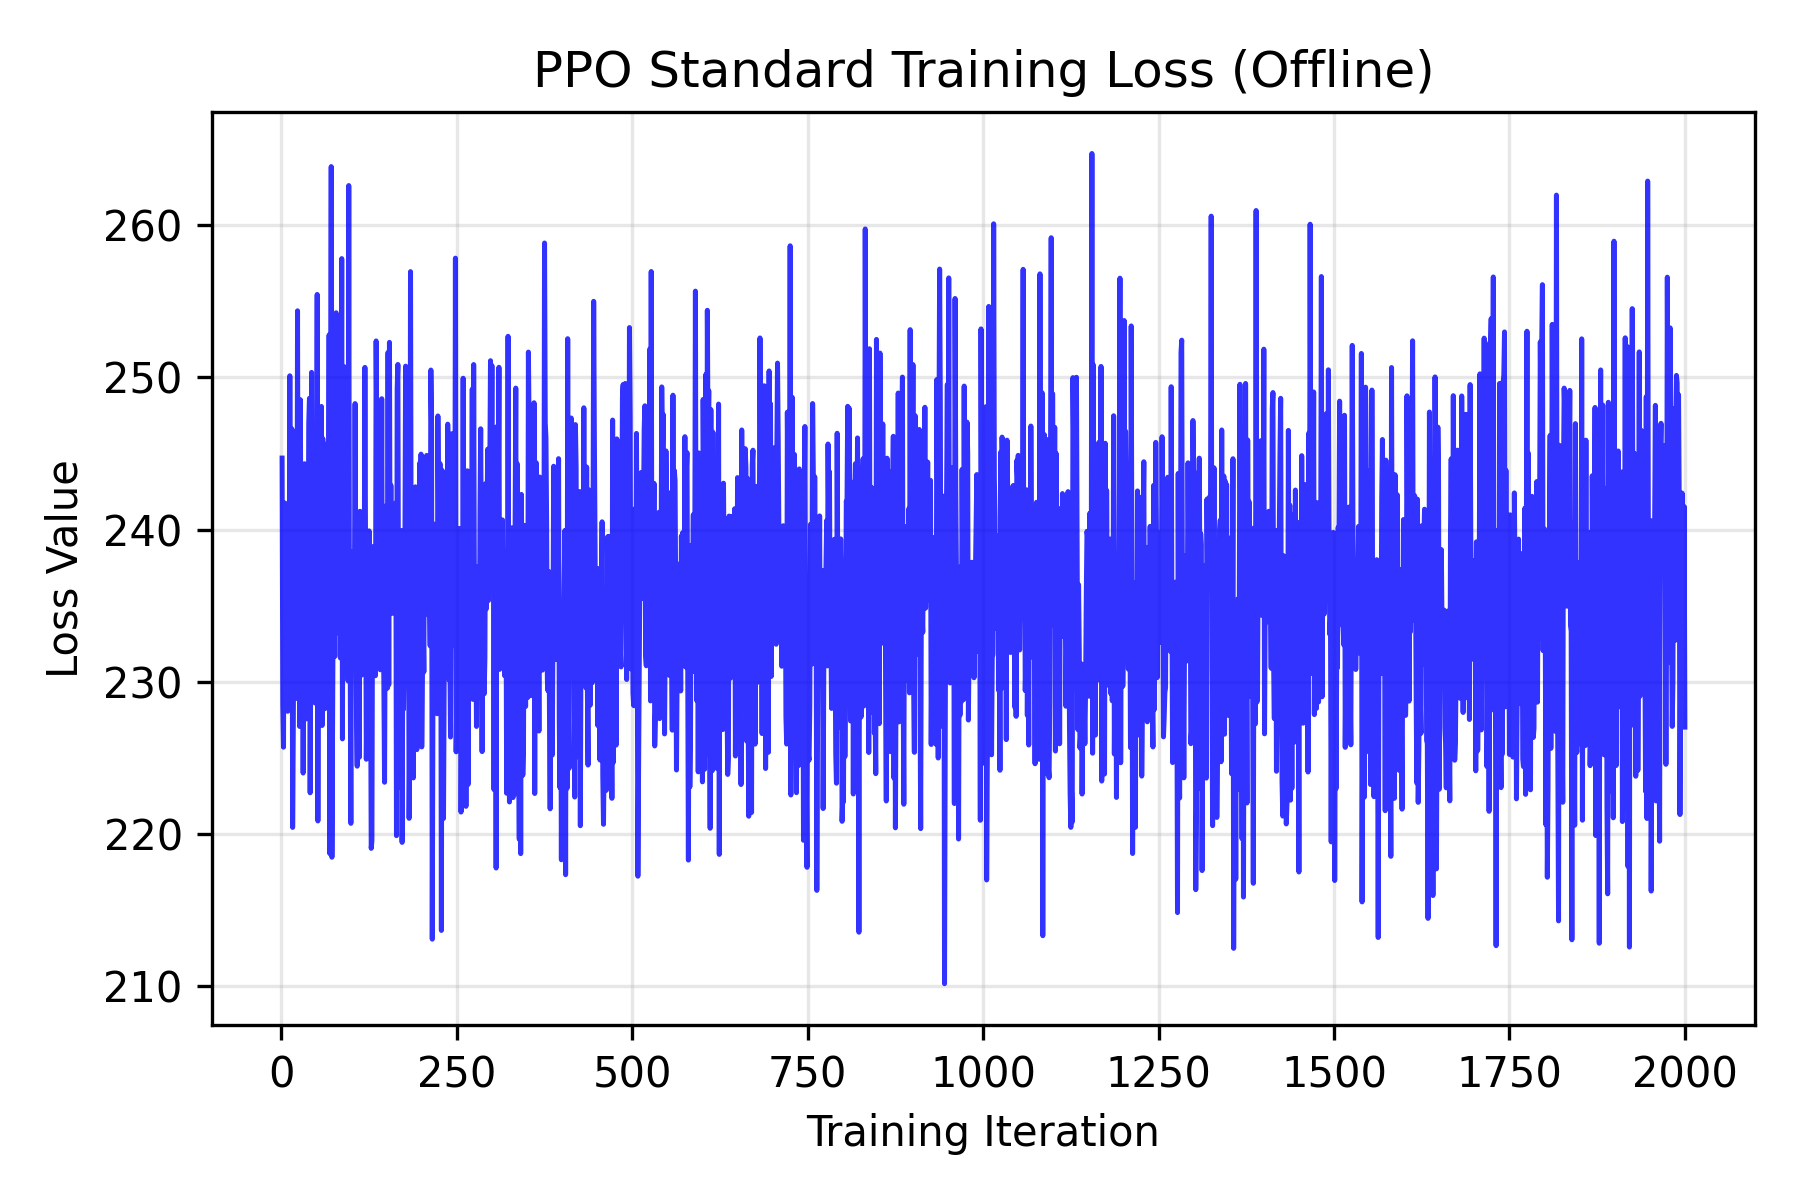
\includegraphics[width=\columnwidth]{figures/fig7_ppo_convergence.png}
\caption{PPO Standard Training Loss (Offline).}
\label{fig:7}
\end{figure}


\begin{figure}[htbp]
\centering
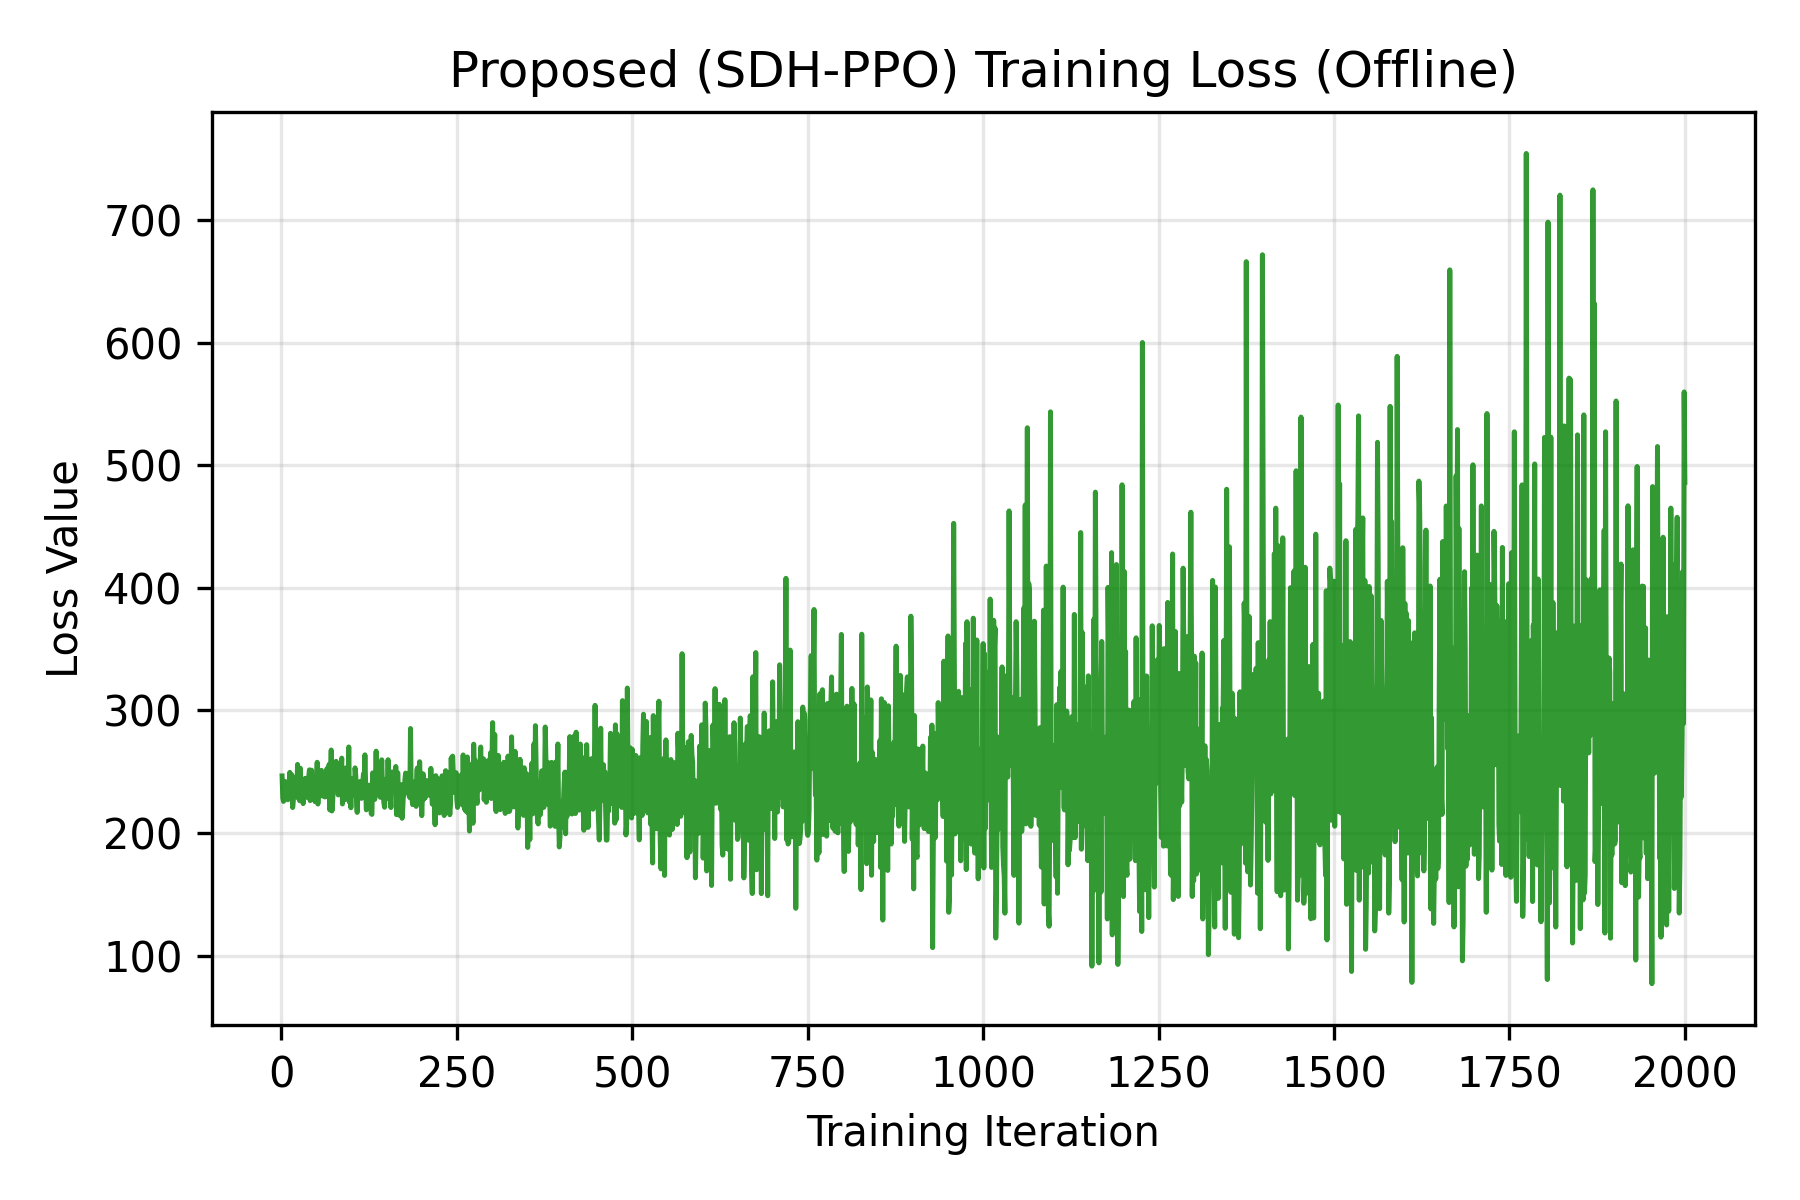
\includegraphics[width=\columnwidth]{figures/fig8_sdh_ppo_convergence.png}
\caption{Proposed SDH-PPO Training Loss (Offline).}
\label{fig:8}
\end{figure}


\section{V. Conclusions}\label{v.-conclusions}

This research has presented the SDH-PPO framework as an autonomous resource orchestration strategy to address the operational challenges in multi-tenant SDN-based IoT environments. By integrating WGAN-GP-based data augmentation, the proposed framework successfully encapsulated latent traffic probability distributions, which significantly enhanced the learning agent\textquotesingle s generalization capabilities across various network slicing scenarios. Experimental results demonstrate that the SDH-PPO framework consistently outperforms baseline methodologies, achieving a superior total violation rate of 27.3\%, representing a performance improvement of more than 47.6\% over standard implementations. Most notably, the framework achieved a 0.0\% violation rate for critical Priority 4 (P4) traffic with a minimal average latency of 2.71 ms, ensuring rigorous adherence to Service Level Agreements (SLAs) for sensitive telemetry. Although the proposed model requires approximately twice the training epochs to converge compared to traditional models, the resulting policy exhibits exceptional stability and robustness in its reward acquisition process. Ultimately, these findings validate the efficacy of the SDH-PPO framework as a reliable and adaptive solution for dynamic resource management in next-generation IoT infrastructures.

\begin{thebibliography}{39}
\bibitem{b1} S. Wijethilaka and M. Liyanage, ``Survey on Network Slicing for Internet of Things Realization in 5G Networks,'' Apr. 01, 2021, \emph{Institute of Electrical and Electronics Engineers Inc.} doi: 10.1109/COMST.2021.3067807.

\bibitem{b2} V. Sharma, ``Performance Evaluation of Network Slicing in 5G Core Networks,'' \emph{International Journal of Multidisciplinary Research and Growth Evaluation}, vol. 3, no. 5, pp. 648--654, 2022, doi: 10.54660/.ijmrge.2022.3.5.648-654.

\bibitem{b3} E. Thomatos, A. Sgora, A. Tsipis, and P. Chatzimisios, ``AI Methods in Network Slice Life-Cycle Phases: A Survey,'' Oct. 01, 2025, \emph{Multidisciplinary Digital Publishing Institute (MDPI)}. doi: 10.3390/electronics14204053.

\bibitem{b4} W. He, H. Yao, H. Chang, and Y. Liu, ``A P4-Based Approach to Traffic Isolation and Bandwidth Management for 5G Network Slicing,'' \emph{Tsinghua Sci. Technol.}, vol. 30, no. 1, pp. 171--185, Sep. 2024, doi: 10.26599/tst.2024.9010020.

\bibitem{b5} Y. Safaei, P. Arefijamal, M. Siamaki, and B. Safaei, ``Priority-Aware SDN Orchestration for Surgical IoMT: A Joint Optimization of Hit Ratio and Latency With Dynamic Resource Reallocation,'' \emph{IEEE Access}, vol. 13, pp. 113787--113808, 2025, doi: 10.1109/ACCESS.2025.3583899.

\bibitem{b6} V. Onaji, E. Adediji, J. Njimgou, K. Ayano, and D. Olufemi, ``Deep Reinforcement Learning for Dynamic Network Slicing and Resource Orchestration in Software-Defined Critical Telecom Infrastructure,'' \emph{International Journal of Computer Applications Technology and Research}, Nov. 2025, doi: 10.7753/ijcatr1411.1006.

\bibitem{b7} P. Jangale~ , ``Impact of Network Slicing on Performance in 5G and Beyond,'' \emph{Journal of Artificial Intelligence, Machine Learning and Data Science}, vol. 1, no. 1, pp. 1653--1657, Nov. 2022, doi: 10.51219/jaimld/pratik-jangale/368.

\bibitem{b8} S. T. Arzo \emph{et al.}, ``MSN: A Playground Framework for Design and Evaluation of MicroServices-Based sdN Controller,'' \emph{Journal of Network and Systems Management}, vol. 30, no. 1, Jan. 2022, doi: 10.1007/s10922-021-09631-7.

\bibitem{b9} R. Pérez, M. Rivera, Y. Salgueiro, C. R. Baier, and P. Wheeler, ``Moving Microgrid Hierarchical Control to an SDN-Based Kubernetes Cluster: A Framework for Reliable and Flexible Energy Distribution,'' \emph{Sensors}, vol. 23, no. 7, Apr. 2023, doi: 10.3390/s23073395.

\bibitem{b10} V. Kumar Sharma, ``Cloud-Native 5G Deployments: Kubernetes and Microservices in Telco Networks,'' \emph{International Journal of Innovative Research in Engineering \& Multidisciplinary Physical Sciences}, vol. 10, no. 3, pp. 1--8, 2022, {[}Online{]}. Available: www.ijirmps.org

\bibitem{b11} A. Kamisetty, D. Narsina, M. Rodriguez, S. Kothapalli, J. Chandra, and S. Gummadi, ``Microservices vs. Monoliths: Comparative Analysis for Scalable Software Architecture Design,'' \emph{Engineering International}, vol. 11, no. 2, 2023.

\bibitem{b12} S. T. Arzo, D. Scotece, R. Bassoli, M. Devetsikiotis, L. Foschini, and F. H. P. Fitzek, ``Softwarized and containerized microservices-based network management analysis with MSN,'' \emph{Computer Networks}, vol. 254, Dec. 2024, doi: 10.1016/j.comnet.2024.110750.

\bibitem{b13} Y. Xu and Q. Yu, ``Deep reinforcement learning based computation offloading and resource allocation strategy for maritime internet of things,'' \emph{Computer Networks}, vol. 264, Jun. 2025, doi: 10.1016/j.comnet.2025.111221.

\bibitem{b14} B. M. Alrifai, L. Alsbatin, and F. Zawaideh, ``Optimizing 5G Resource Allocation with Reinforcement Learning: A Q-Learning and Deep Q-Network (DQN) Approach,'' \emph{Journal of Advances in Information Technology}, vol. 16, no. 11, pp. 1586--1594, 2025, doi: 10.12720/jait.16.11.1586-1594.

\bibitem{b15} M. Hosseinzadeh \emph{et al.}, ``SDN-Based NFV deployment for multi-objective resource allocation in edge computing: A deep reinforcement learning for iot workload scheduling,'' \emph{Sustainable Computing: Informatics and Systems}, vol. 48, Dec. 2025, doi: 10.1016/j.suscom.2025.101218.

\bibitem{b16} V. Sittakul, I. Ioannou, P. Nagaradjane, and V. Vassiliou, ``Intelligent congestion control in 5G URLLC Software-Defined Networks using adaptive resource management via Reinforced Dueling Deep Q-Networks,'' \emph{Journal of Network and Computer Applications}, vol. 242, Oct. 2025, doi: 10.1016/j.jnca.2025.104276.

\bibitem{b17} A. Iqbal, A. Nauman, T. Khurshaid, and S. B. Rhee, ``A Scalable Reinforcement Learning Framework for Ultra-Reliable Low-Latency Spectrum Management in Healthcare Internet of Things,'' \emph{Mathematics}, vol. 13, no. 18, Sep. 2025, doi: 10.3390/math13182941.

\bibitem{b18} M. Chahoud \emph{et al.}, ``Reward shaping in DRL: A novel framework for adaptive resource management in dynamic environments,'' \emph{Inf. Sci. (N. Y).}, vol. 715, Oct. 2025, doi: 10.1016/j.ins.2025.122238.

\bibitem{b19} A. Abderrahmane, H. Drid, and A. Behaz, ``A Survey of Controller Placement Problem in SDN-IoT Network,'' Dec. 01, 2024, \emph{Springer Science and Business Media B.V.} doi: 10.1007/s44227-024-00035-y.

\bibitem{b20} R. Botez, J. Costa-Requena, I. A. Ivanciu, V. Strautiu, and V. Dobrota, ``Sdn-based network slicing mechanism for a scalable 4g/5g core network: A kubernetes approach,'' \emph{Sensors}, vol. 21, no. 11, Jun. 2021, doi: 10.3390/s21113773.

\bibitem{b21} J. M. Fernandez, I. Vidal, and F. Valera, ``Enabling the orchestration of IoT slices through edge and cloud microservice platforms,'' \emph{Sensors (Switzerland)}, vol. 19, no. 13, Jul. 2019, doi: 10.3390/s19132980.

\bibitem{b22} Y. Zhang, C. Li, N. Chen, and P. Zhang, ``Intelligent Requests Orchestration for Microservice Management Based on Blockchain in Software Defined Networking: A Security Guarantee,'' in \emph{2022 IEEE International Conference on Communications Workshops, ICC Workshops 2022}, Institute of Electrical and Electronics Engineers Inc., 2022, pp. 254--259. doi: 10.1109/ICCWorkshops53468.2022.9814536.

\bibitem{b23} F. Tonini, C. Natalino, M. Furdek, C. Raffaelli, and P. Monti, ``Network Slicing Automation: Challenges and Benefits,'' in \emph{2020 24th International Conference on Optical Network Design and Modeling, ONDM 2020}, 2020. doi: 10.23919/ONDM48393.2020.9133004.

\bibitem{b24} S. Sriharsha Rachakonda and R. Lakshmikanth, ``Enhancing Network Security With Qos-Aware Optimization Models In 6G Network Slicing Architectures.'' {[}Online{]}. Available: https://www.theaspd.com/ijes.php

\bibitem{b25} P. Kochovski, U. Paščinski, V. Stankovski, and M. Ciglarič, ``Pareto-Optimised Fog Storage Services with Novel Service-Level Agreement Specification,'' \emph{Applied Sciences (Switzerland)}, vol. 12, no. 7, Apr. 2022, doi: 10.3390/app12073308.

\bibitem{b26} K. Zia, A. Chiumento, P. Havinga, R. Riggio, and Y. Huang, ``QoS Aware Slice Resource Management Using Deep Reinforcement Learning in IoT Networks,'' in \emph{2023 19th International Conference on Distributed Computing in Smart Systems and the Internet of Things (DCOSS-IoT)}, Jan. 2023, pp. 150--154. doi: 10.1109/DCOSS-IoT58021.2023.00035.

\bibitem{b27} F. Mason, G. Nencioni, and A. Zanella, ``Using Distributed Reinforcement Learning for Resource Orchestration in a Network Slicing Scenario,'' \emph{IEEE/ACM Transactions on Networking}, vol. 31, no. 1, pp. 88 -- 102, 2023, doi: 10.1109/TNET.2022.3187310.

\bibitem{b28} S. Venkatapathy, T. Srinivasan, O. S. Lee, R. Jayaraman, H. G. Jo, and I. H. Ra, ``Slice-aware 5G network orchestration framework based on dual-slice isolation and management strategy (D-SIMS),'' \emph{Sci. Rep.}, vol. 14, no. 1, Dec. 2024, doi: 10.1038/s41598-024-68892-9.

\bibitem{b29} H. She, L. Yan, X. An, C. Mao, and Y. Guo, ``Flow persona: A QoS Flow Rule Scheme based on Deep Learning in SDN-IoT,'' \emph{Computer Networks}, vol. 273, 2025, doi: 10.1016/j.comnet.2025.111784.

\bibitem{b30} A. Holscher, M. Asplund, and F. Boeira, ``Evaluation of an SDN-based Microservice Architecture,'' in \emph{Proceedings of the 2022 IEEE International Conference on Network Softwarization: Network Softwarization Coming of Age: New Challenges and Opportunities, NetSoft 2022}, 2022, pp. 151 -- 156. doi: 10.1109/NetSoft54395.2022.9844094.

\bibitem{b31} M. Zambianco and G. Verticale, ``Intelligent multi-branch allocation of spectrum slices for inter-numerology interference minimization,'' \emph{Computer Networks}, vol. 196, 2021, doi: 10.1016/j.comnet.2021.108254.

\bibitem{b32} M. F. Ul Islam, S. Hossain, M. G. R. Alam, N. Mansoor, and A. Chakrabarty, ``Optimizing network bandwidth slicing identification: NADAM-enhanced CNN and VAE data preprocessing for enhanced interpretability,'' \emph{PLoS One}, vol. 20, no. 10 October, Oct. 2025, doi: 10.1371/journal.pone.0333286.

\bibitem{b33} L. Zhao, Y. Liu, A. Hawbani, N. Lin, W. Zhao, and K. Yu, ``QoS-Aware Multihop Task Offloading in Satellite--Terrestrial Edge Networks,'' \emph{IEEE Internet Things J.}, vol. 11, no. 19, pp. 31453--31466, Oct. 2024, doi: 10.1109/JIOT.2024.3417456.

\bibitem{b34} C. Ssengonzi, O. P. Kogeda, and T. O. Olwal, ``A survey of deep reinforcement learning application in 5G and beyond network slicing and virtualization,'' \emph{Array}, vol. 14, 2022, doi: 10.1016/j.array.2022.100142.

\bibitem{b35} T. Mai, H. Yao, N. Zhang, W. He, D. Guo, and M. Guizani, ``Transfer Reinforcement Learning Aided Distributed Network Slicing Optimization in Industrial IoT,'' \emph{IEEE Transactions on Industrial Informatics}, vol. 18, no. 6, pp. 4308--4316, Jun. 2022.

\bibitem{b36} D. H. Abdulazeez and S. K. Askar, ``Offloading Mechanisms Based on Reinforcement Learning and Deep Learning Algorithms in the Fog Computing Environment,'' \emph{IEEE Access}, vol. 11, pp. 12554--12585, 2023, doi: 10.1109/ACCESS.2023.3241881.

\bibitem{b37} C. Tan, ``Comparative Study of Reinforcement Learning Performance Based on PPO and DQN Algorithms,'' \emph{Applied and Computational Engineering}, vol. 175, pp. 30--36, 2025.
\bibitem{b38} M. Arjovsky, S. Chintala, and L. Bottou, ``Wasserstein Generative Adversarial Networks,'' in \emph{Proceedings of the 34th International Conference on Machine Learning (ICML)}, PMLR, 2017, pp. 214--223. Available: https://dl.acm.org/doi/10.5555/3305381.3305404
\bibitem{b39} I. Gulrajani, F. Ahmed, M. Arjovsky, V. Dumoulin, and A. Courville, ``Improved Training of Wasserstein GANs,'' in \emph{Advances in Neural Information Processing Systems (NeurIPS)}, vol. 30, 2017. Available: https://papers.nips.cc/paper\_files/paper/2017/hash/892c3b1c6dccd52936e27cbd0ff683d6-Abstract.html

~
\end{thebibliography}

\end{document}
